
\documentclass[12pt,a4paper,titlepage]{article}
\usepackage{license_style}


\usepackage[style=numeric-comp, backend=bibtex, sorting=none]{biblatex}
\addbibresource{thesis.bib}

\begin{document}

\pagenumbering{gobble} % disable page numbering

% TODO: INCLUDE TITLE PAGES

\section*{Abstract}

This thesis represents an attempt to use modern web technology in the field of
real-time communication in order to enhance and encourage communication and
interaction between humans. It is to be done by the development of a web-based
multiplayer game that uses mobile phones as wireless controllers in order to
emulate the experience of a gaming console.

The text of the thesis consists of four chapters that encompass individual steps
of the project's development process. Chapter 1 performs an in-depth analysis of
the domain, provides a brief overview of how did human interaction with
computers evolve, and identifies the motivation for the project. In the same
chapter are depicted the potential technologies (WebSockets and WebRTC) that can
be used for solving the problem in question. The last sections of the first
chapter contain an analysis of applications that are currently present on the
market and follow similar ideas.

Chapter 2 is focused on the architectural aspects of the system. It includes the
results of the modeling process in form of UML diagrams with descriptions of the
system and individual parts of it, from different perspectives. Design decisions
are also specified in this chapter, along with the motivations that stood behind
them.

The third chapter provides a detailed insight of the project implementation. The
three major subsections describe respective parts of the system, specifically:
the main game, the controller component and the code that realizes the
communications between these two. Code excerpts with commentaries try to
emphasize the techniques and tools that were used during development.

The last chapter performs an economic overview of the project with the attempt
to estimate its market potential. It includes calculations of various types of
expenses that result in the total product cost. This is used to compute the
economic indicators of the project and the retail price of the individual unit
of the product if it had to be sold on the market.

At the end of the thesis, the conclusion presents the outcomes of the project
and the general results gain during the work with the technologies used in the
development process.


\clearpage


\section*{Rezumat}

\selectlanguage{romanian}

Această teză reprezintă o încercare de a utiliza tehnologiile web moderne și
anume acelea din domeniul comunicării în timp real, cu scopul de a consolida și
de a încuraja comunicarea și interacțiunea între oameni. Scopul va fi realizat
prin dezvoltarea unui joc multiplayer bazat pe web ce utilizează telefoanele
mobile în calitate de dispozitiv de control, emulînd experiența unei
console de jocuri.

Textul tezei este format din patru capitole, care cuprind etapele individuale a
procesului de dezvoltare a proiectului. Capitolul 1 efectuează o analiză
detaliată a domeniului, oferă un scurt istoric a modului în care a evoluat
interacțiunea omului cu calculatorul și identifică motivația pentru proiectul
tezei. În același capitol sunt prezentate potențialele tehnologii (WebSockets și
WebRTC) ce pot fi utilizate pentru rezolvarea problemei în cauză. Ultimele
secțiuni ale primului capitol conțin o analiză a aplicațiilor care sunt în
prezent pe piață.

Capitolul 2 este axat pe aspectele arhitecturale ale sistemului. El include
rezultatele procesului de modelare în formă de diagrame UML, însoțite de
descrierea sistemului și a părților individuale a acestuia din diferite
perspective. La fel sunt specificate deciziile de proiectare, împreună cu
motivațiile care au stat în spatele lor.

Al treilea capitol oferă o perspectivă detaliată asupra implementării
proiectului. Trei subsecțiuni majore descriu părțile respective ale sistemului,
și anume: jocul, componenta dispozitivului de joc și codul care realizează
comunicarea între acestea. La fel sunt incluse fragmente de cod cu comentarii ce
accentuează tehnicile și instrumentele care au fost folosite în timpul
dezvoltării.

Ultimul capitol realizează o trecere în revistă a proiectului din punct de
vedere economic cu încercarea de a estima potențialul său economic. Acesta
include calcule de diferite tipuri de cheltuieli care în ansamblu constituie
costul total al produsului. Acesta este folosit pentru a calcula indicatorii
economici ai proiectului și prețul de vânzare a unei unități de
produs în cazul în care acesta ar fi introdus pe piață.

La finalul tezei sunt prezentate rezultatele generale a proiectului care au fost
obținute în timpul lucrului cu tehnologiile utilizate în proces de dezvoltare.

\selectlanguage{english}

\clearpage



\tableofcontents
\clearpage

\pagenumbering{arabic} % re-enable page numbering
\setcounter{page}{10} % TODO: FIX PAGE NUMBERING



\phantomsection
\addcontentsline{toc}{section}{List of figures}
\listoffigures
\clearpage


% \phantomsection
% \addcontentsline{toc}{section}{List of tables}
% \listoftables
% \clearpage


\phantomsection
\addcontentsline{toc}{section}{Listings}
\numberwithin{lstlisting}{section}
\lstlistoflistings
\clearpage


\phantomsection
\addcontentsline{toc}{section}{Introduction}
\section*{Introduction}




\clearpage


\section{Domain Analysis}

\subsection{User Interfaces and Input Devices}

% Before diving in the deeps of real-time communication over the Web, it is necessary to review the path that people took in order to interact with computers in the first place.

At the very beginning of the computer era, the devices that we now know as
PCs, laptops and tablets were immense pieces of machinery that occupied entire
laboratories and only highly qualified individuals had access to them. These
machines where developed in order to perform various numerical problems by
executing digital computations. As the saying goes, a machine can only do what
a man tells it to do, so engineers had to come up with different means to set
tasks for these electronic beasts, that is, a need for \emph{user interfaces}
arouse. Operators used large stacks of punched cards to feed instructions and
data sets to computers. These punched cards in turn where created using
specialized devices that also required some knowledge in the field. Over all
it was a complex process that couldn't be easily grasped by an ordinary
persons. At that time, however, the majority of computer user had PhDs and
were trained to perform these very tasks so the difficulty of communicating
with machines wasn't really a great problem.

% picture of ENIAC maybe

In time, the interest towards computers grew bigger among enthusiasts while
the devices themselves where becoming smaller and smaller, eventually giving
birth to the term of 'microcomputer'. Among the first microcomputers to get
widespread popularity was the critically acclaimed Altair 8080 which
represented a box with lights and switches on the front panel that where used
to feed data and instructions into the computer and read the results back from
it.

% picture of Altair 8080 front panel

As more hobbyists took a hold of such devices people discovered many uses for
them beyond that of performing various mathematical operations. They learned
how to connect teletypes to computers and this way the later got an interface
that is familiar to all of us today, a keyboard. For some time people
interacted with computers using command lines, but with the development of
computer graphics and the creation of graphical user interfaces, a need for a
new kind of controller appeared, specifically the need for a pointing device.
Since then, a standard personal computer included a mouse and a keyboard among
it's peripheral devices.

\subsubsection{Input Devices for Gaming}

On the other hand, the development of input devices never stopped with the
creation of the mouse and keyboard. A wealth of specialized devices was
created to perform tasks that were specific to a particular use of the
computer. One of the most notable fields that was moving the development of
specialized peripherals was and still is the \emph{game development industry}.
During the years, various types of controllers were developed, some of them
are listed below:

\begin{description}

    \item [Gamepad] is a general-purpose gaming device that is used as a
        controller for a wide range of game genres, from arcades and fighting
        games to role-playing titles and action third-person shooters.

    \item [Joystick] is a specialized controller that is often used in flight
        simulation games, although its use can be extended far beyond gaming, for such
        purposes as remote control of a robot arm in a warehouse.

    \item [Steering Wheel] is used to provide almost authentic driving
        experience in racing video games.

\end{description}


\begin{figure}[!ht]
    \centering
    \subfloat[Gamepad\label{fig:gamepad}]{
      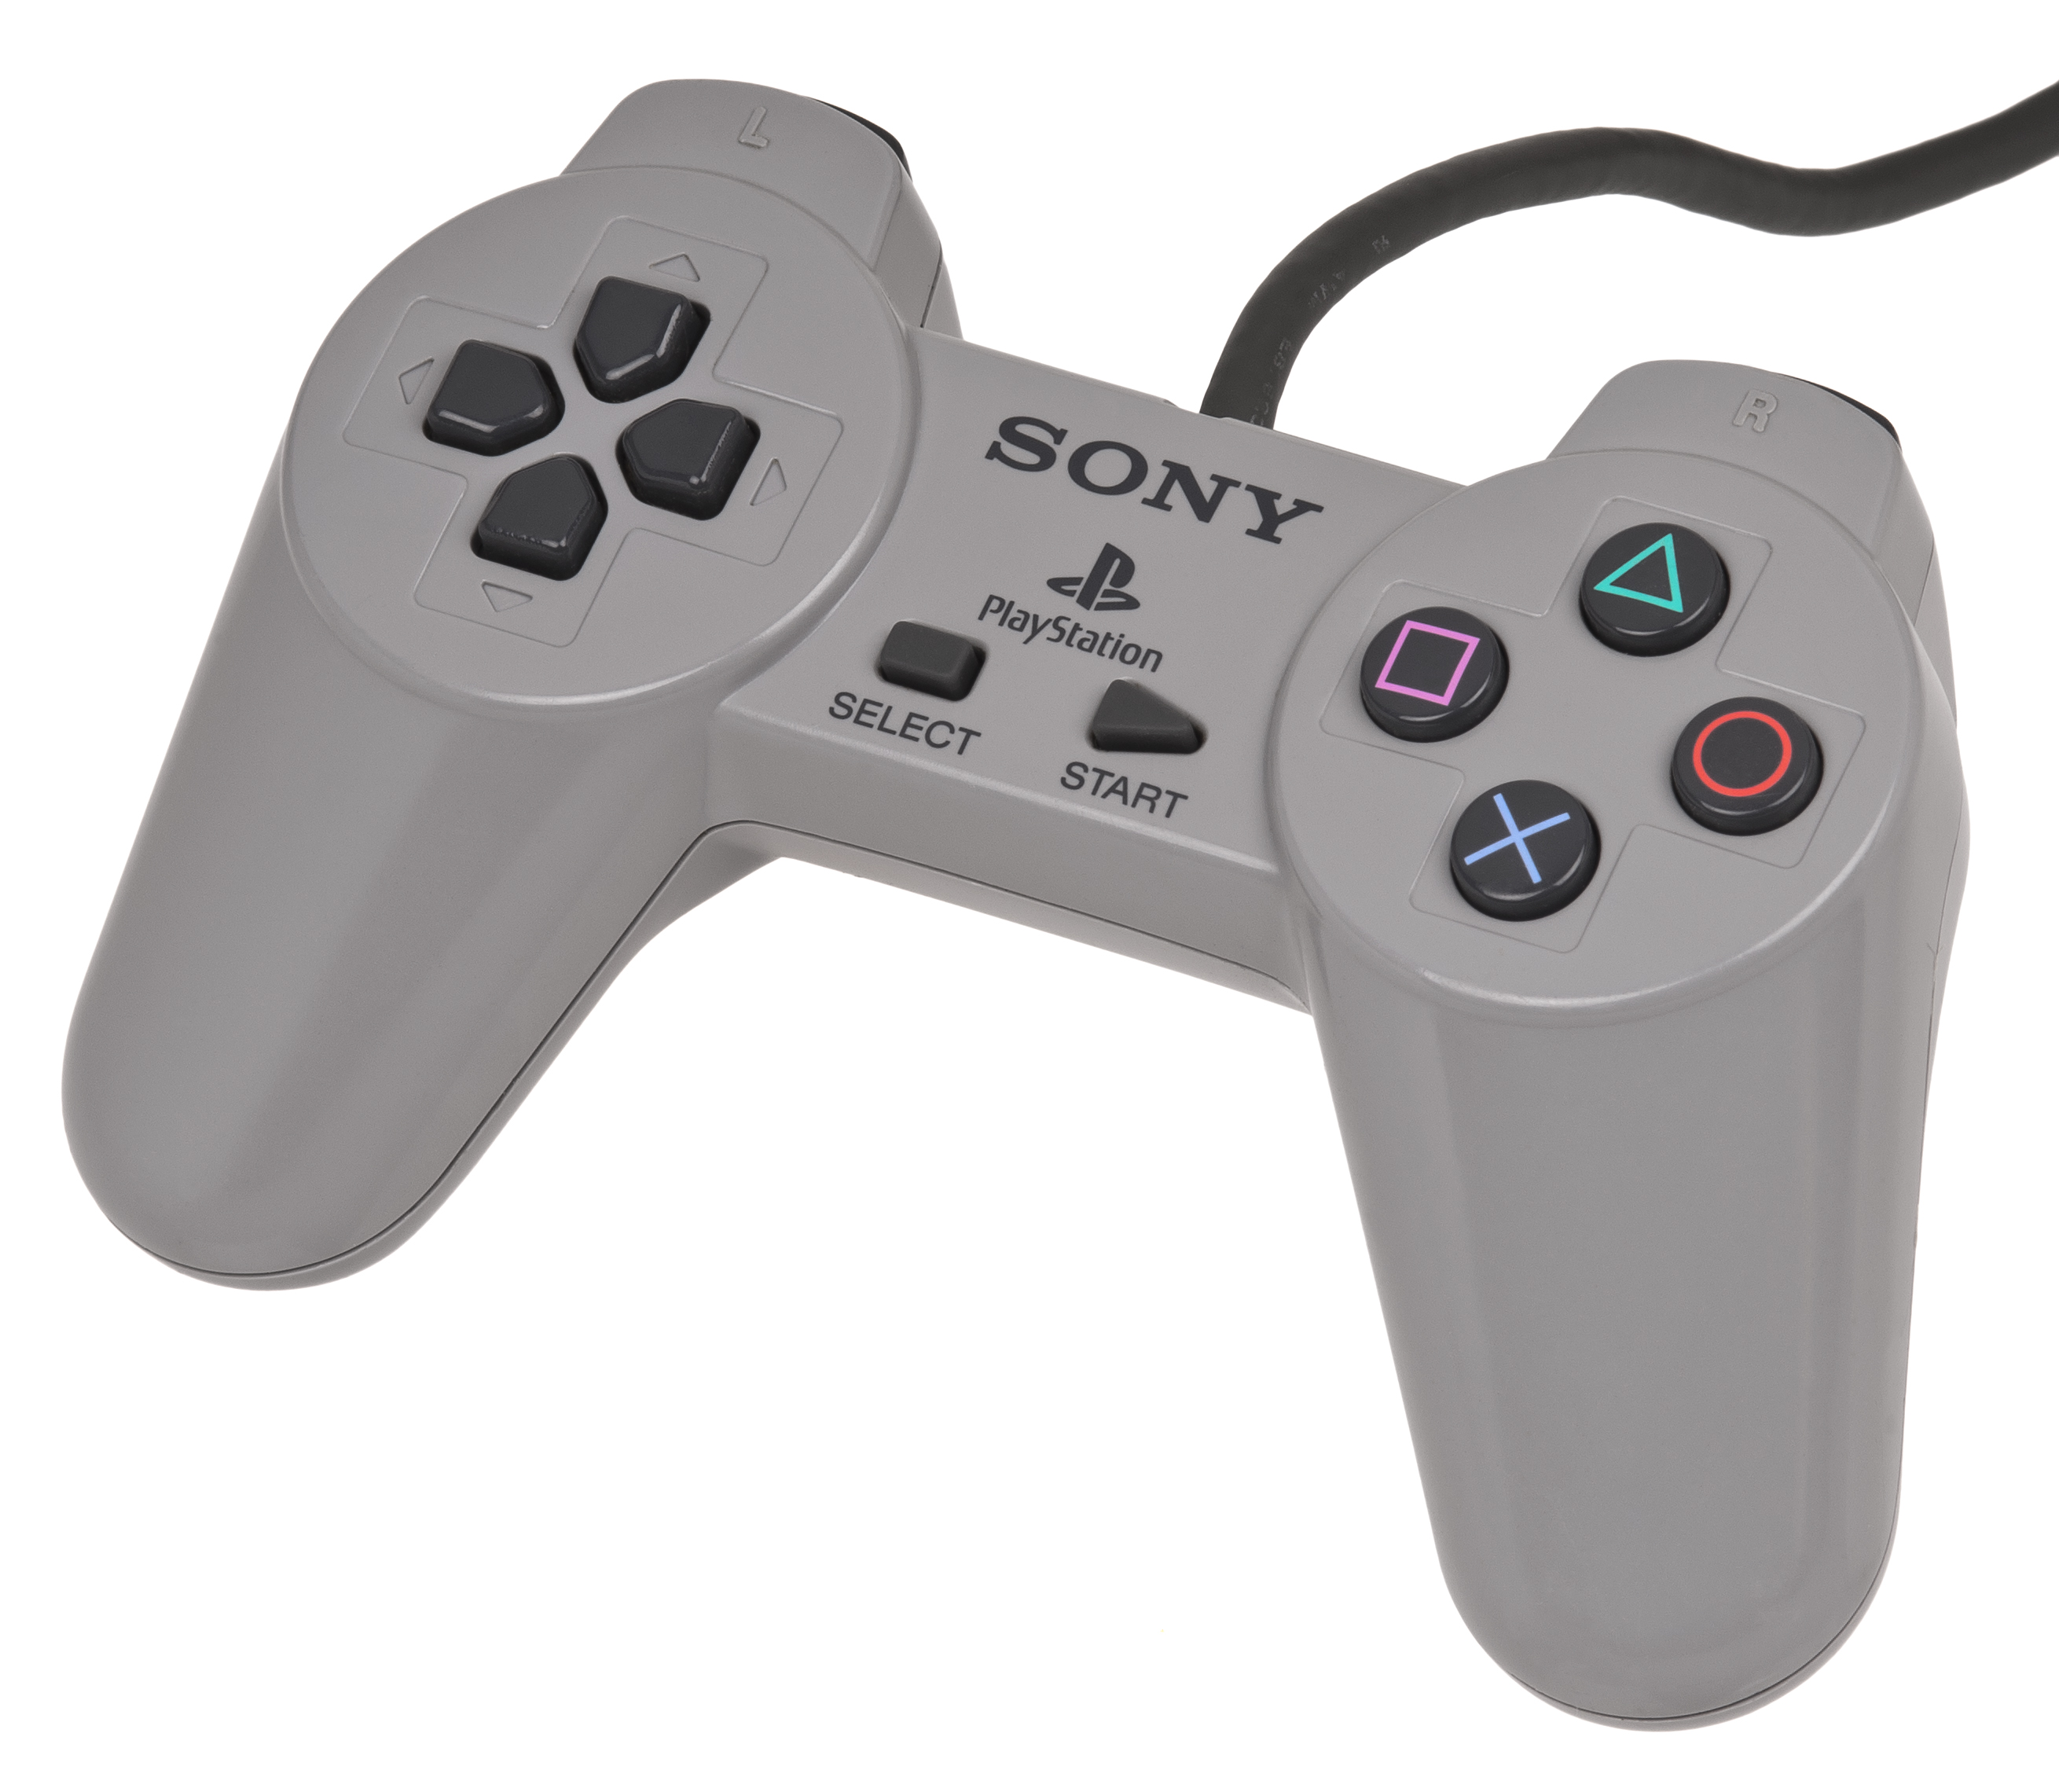
\includegraphics[width=0.3\textwidth]{ps_controller}
    }
    \subfloat[Steering Wheel Controller\label{fig:wheel}]{
      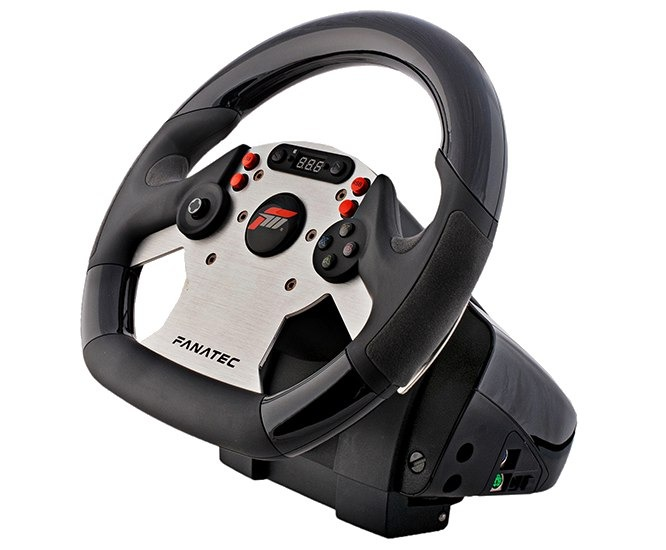
\includegraphics[width=0.3\textwidth]{steering_wheel}
    }
    \subfloat[Joystick\label{fig:joystick}]{
      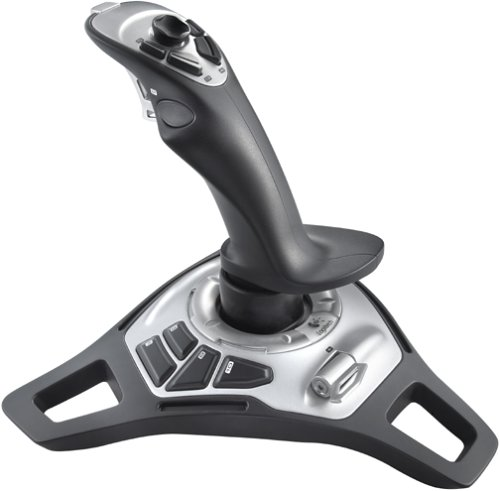
\includegraphics[width=0.3\textwidth]{logitech_joystick}
    }
    \caption{Examples of Input Devices for Gaming}
\end{figure}



\subsection{Mobile User Interfaces}

Very soon, technological progress made it possible to stick microcomputers
virtually in any device, be it a fridge, microwave oven or a car. The most
benefit out of this, however, gained the industry of mobile phones, eventually
giving birth to the concept of smart-phones. Today, almost every person living
in a more or less civilized region of the world has in his/her pocket a little
'brick' with the computer power thousands of times greater than the one that
was used to send people to the moon. This breakthrough in portable computing
facilitated the development of software for such devices and the majority of
companies started to support mobile applications where it made sense.

In the context of user interface design and input handling techniques,
developers found themselves in a completely different world. Nobody would
carry a mouse and a keyboard in order to interact with the phone, instead,
people would use the number pad plus a couple of additional buttons present on
the phone. In time, another revolution took place, it was the moment when
touch screens became reality. Once again, developers had to think their way
through these changes and create user interfaces that would suit fingers
poking into the screen rather than button clicks. With the difficulties of
user interface redesign for touch devices came also a wide range of new
possibilities. Now that the whole screen constituted an input device, the
users could perform gestures like taps, swipes, pan motions, pinch-zoom
actions. These gestures made the process of using an application a great deal
more intuitive when compared to the times when every action was performed
through the click of a certain button.

Besides touch screens, mobile phone vendors began to include in their devices
such sensors like accelerometers and gyroscopes. Accelerometers are used to
catch the moment when the device is moved and to calculate the direction and
acceleration of such movement. On the software side this could be used in
various ways, the simplest being to switch to the next song in the music
player by jerking the phone to the right. Meanwhile, gyroscopes where designed
to capture the orientation of the device at a given moment in time. This
functionality is employed every time the phone is tilted over 90 degrees and
triggers the switch between landscape and portrait view modes.

\newpage

When it came to the industry of mobile gaming, touch screens and sensors that
could capture the motion and orientation of the device were a really big deal,
because they opened the possibilities for developing complex user interfaces
that would simulate specialized gaming devices. The accelerometer and
gyroscope would be used as the steering wheel in racing games while the touch
screen would capture taps in various regions and interpret them as clicks of
different buttons of a gamepad, whose simplified image would be rendered on
the same screen.

% picture of mobile game UI which resembles a gamepad

\subsection{Mobile Devices as Controllers for Desktop Computers}

When comparing the features of a specialized gaming device like \emph{Nintendo
Wii}\cite{wiimote} Controller and the capabilities of a modern smart-phone, an interesting
pattern of similarities can be observed. Both are able to capture device
motion and position. Both respond to clicks of buttons in case of a gamepad
and taps in designated areas in case of a phone. Touch screens can be used to
simulate even the motion of a joystick, by capturing swipe or pan gestures.
One feature that a specialized gaming device may have, that a phone falls
short of, is ergonomics, but to a certain extent this can be neglected. With
such a list of similarities, a logical question appears: Why not use mobile
phones as gaming controllers for desktop games?


\subsubsection{Usability Limitations}

As it turns out, now that smart-phones run full-fledged operating systems,
connecting one to a computer is not that hard of a task. Mobile operating
systems like Android, Apple iOS and Windows Mobile, all support socket
programming, thus a programmer can setup a communication channel over the
network between a mobile phone and a laptop connected to the same Wi-Fi
hotspot. They can even be located on different sides of the planet, it is
sufficient to have an Internet connection to be able to exchange data between
devices.

Overall it looks like a way to go approach. On the other hand, there are some
problems with it that are not to be observed at first sight. In the first
place, every time that a company wants to create a game with support for
mobile devices as controllers, the developers will have to write custom mobile
applications in addition to the main game, they will also have to devise
specialized communication protocols. This is both, time and money consuming
and is not economically convenient. Secondly, there is a problem on the user
side which is best illustrated with a situation. Let's suppose a party or a
team-building event where the host tries to entertain his guests with a
multiplayer computer game. Not everyone has at home a gaming platform like
Sony Playstation or Microsoft Xbox, neither does anyone have more than 2-3 PC
gamepads. In this situation, the ability to use smart-phones as controllers
would be a great benefit. In case the connection is implemented in the way
described above, a gaming party would transform into a setup party, where
guests would spend a lot of time installing mobile applications that are
probably needed only for one-time use and don't hold any value by themselves
without the main game. Fortunately both problems can be solved relatively
simple through the same solution.

\newpage

\subsubsection{Web-based Workaround}

One thing that all modern smart-phones have in common is a decent web browser.
Today, browsers are more than just viewers of HTML documents, they are entire
ecosystems and programming environments that are almost independent of the
underlying operating system. The fact that every mobile phone has such an
environment makes it possible to write cross-platform application served on
the web that would otherwise be installed manually as a native app. Modern
browsers support APIs that can interact with various parts of a mobile device
like accelerometer, gyroscope and touch screen, exactly the things that are
necessary to simulate a fully functional gaming device.

Having said this, one thing that could solve the problems stated in the
section above may be a framework or toolkit that unifies in a single library
all the APIs that are necessary to connect a mobile phone to a computer as a
remote gaming controller. It would make it easier and faster to develop games
with such a feature. This toolkit may also include user interface building
blocks which can be combined to create custom controllers.

The purpose of this thesis is to create a simple web-based multiplayer
isometric arcade called 'Snowfight'. The main game is started by accessing its
web page. The first thing the players see is a lobby and a connection URL.
Players join the game by navigating to the provided URL using the browsers
installed on their phones. When enough players have connected and the
participants decide to start the game, a button can be clicked on the main
game screen. The game play concept is rather simple, players can move their
characters around the game space and throw snowballs in each other using the
controls rendered by the web application that works on their phones. Every
player has a certain amount of hit points (HP) and if a player is hit, his HP
amount decreases. When a player's HP amount reaches zero, he is eliminated
from the game. The goal of the game is to eliminate all players from the
adversary team.

In order to implement this project it is necessary to explore the topic of
real-time communication in the web, as to be able to chose the right technology
that would provide a smooth and responsive gaming experience.


\subsection{Real-Time Communication over the Web}

One of the main uses of the Internet is hosting and accessing web pages. When a
user writes a URL in the browser's search bar and presses 'enter', the browser
preforms an HTTP request to the server specified by the URL and fetches a web
page. At this point in time, for most cases, the communication between the
server and the client (browser) is ceased until the user clicks on another link
that would restart the process.

On the other hand, modern web has greatly developed during the past few years.
Internet connection speed has increased dramatically, and many websites have
stopped being just static web pages and have moved towards a more dynamic model.
They are not even called websites, today, all around the world there are web
applications.

With the requirements for a more dynamic web came also the technical challenges
of making it so. For instance, how would a user's browser receive a notification
about a message that was sent to this user from another part of the globe? When
such questions just appeared, developers tried different techniques using the
old tools they had at hand at that time. The concepts of HTTP Long Polling and
HTTP Streaming appeared in this period. Soon, however, they were found to be
causing quite a bit of issues\cite{long_polling_issues} and a need for custom
protocols arose.

As the web is mainly composed of clients and servers, the logical outcome was a
protocol that would connect them and would permit bidirectional communication
between the server and its clients, thus WebSockets were proposed. At the same
time, browsers grew and their uses extended. Soon, real-time communication out-
sized the context of client-server architecture and when video chat applications
and multiplayer games started to conquer the web realm, engineers developed
WebRTC, which solved the issue of communication in peer-to-peer setups. A brief
description of both protocols as per their RFCs is presented in the sections
that follow.

\subsubsection{WebSockets for Client-Server Communication} % Websockets

Historically, creating web applications that need bidirectional communication
between a client and a server (e.g., instant messaging and gaming applications)
has required an abuse of HTTP to poll the server for updates while sending
upstream notifications as distinct HTTP calls.

As RFC6455\cite{websockets} points out, this results in a variety of problems:

\begin{itemize}

\item The server is forced to use a number of different underlying TCP
  connections for each client: one for sending information to the
  client and a new one for each incoming message.

\item The wire protocol has a high overhead, with each client-to-server
  message having an HTTP header.

\item The client-side script is forced to maintain a mapping from the
  outgoing connections to the incoming connection to track replies.

\end{itemize}

A simpler solution would be to use a single TCP connection for traffic in both
directions. This is what the WebSocket Protocol provides. Combined with the
WebSocket API, it provides an alternative to HTTP polling for two-way
communication from a web page to a remote server.

The same technique can be used for a variety of web applications: games, stock
tickers, multiuser applications with simultaneous editing, user interfaces
exposing server-side services in real time, etc.

The WebSocket Protocol is designed to supersede existing bidirectional
communication technologies that use HTTP as a transport layer to benefit from
existing infrastructure (proxies, filtering, authentication). Such technologies
were implemented as trade-offs between efficiency and reliability because HTTP
was not initially meant to be used for bidirectional communication. The
WebSocket Protocol attempts to address the goals of existing bidirectional HTTP
technologies in the context of the existing HTTP infrastructure; as such, it is
designed to work over HTTP ports 80 and 443 as well as to support HTTP proxies
and intermediaries, even if this implies some complexity specific to the current
environment. However, the design does not limit WebSocket to HTTP, and future
implementations could use a simpler handshake over a dedicated port without
reinventing the entire protocol. This last point is important because the
traffic patterns of interactive messaging do not closely match standard HTTP
traffic and can induce unusual loads on some components.

\newpage

\subsubsection{WebRTC for Peer to Peer Communication} % WebRTC

Real-time communication has been on the market for a while, however, it was
implemented mainly in corporate environments as in-house solutions. It was quite
expensive in terms of effort to include such technology in existing projects
especially in the context of the web. In recent years this started to change
with the appearance of various frameworks and APIs.

WebRTC\cite{webrtc_org} is a free, open project that provides browsers and
mobile applications with Real-Time Communications (RTC) capabilities via simple
APIs. The WebRTC components have been optimized to best serve this purpose.
Due to its properties, WebRTC is of particular interest for the development
of the project for the present thesis.

As Sam Dutton points out in his article\cite{webrtc_basics}, WebRTC has now
implemented open standards for real-time, plugin-free video, audio and data
communication. This solves a range of problems relevant to real-time
communications:

\begin{itemize}
    \item Many web services already use RTC, but need downloads, native apps or
        plugins. These includes Skype, Facebook and Google Hangouts.

    \item Downloading, installing and updating plug-ins can be complex, error
        prone and annoying.

    \item Plugins can be difficult to deploy, debug, troubleshoot, test and
        maintain, and may require licensing and integration with complex,
        expensive technology. It's often difficult to persuade people to install
        plugins in the first place.
\end{itemize}

The guiding principles of the WebRTC project are that its APIs should be open
source, free, standardized, built into web browsers and more efficient than
existing technologies. Presently it is capable of enabling efficient
transmission of audio, video and arbitrary data in a peer-to-peer fashion. At
the same time WebRTC still needs servers because of the following
reasons\cite{webrtc_realworld}:

\begin{itemize}

\item For clients to exchange metadata to coordinate communication: this is
called signaling.

\item To cope with network address translators (NATs) and firewalls.

\end{itemize}



\begin{figure}[!h]
\centering
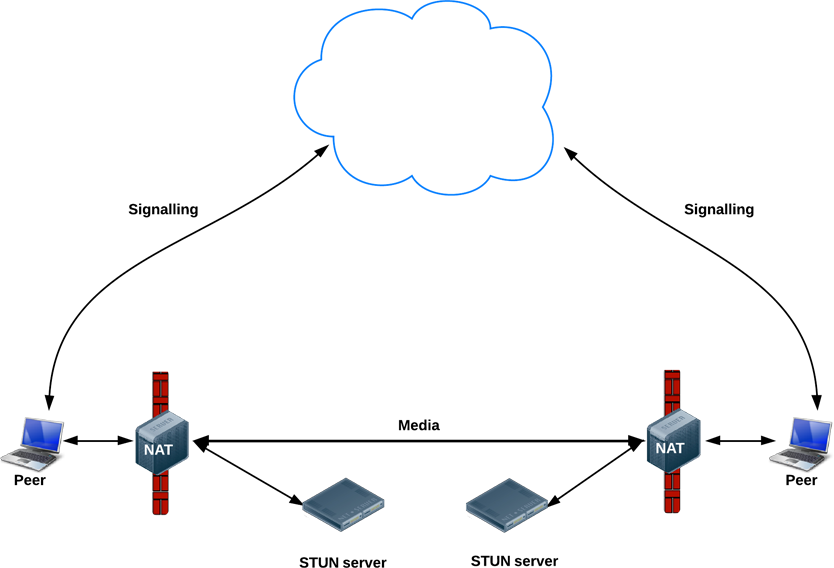
\includegraphics[width=12cm]{webrtc_stun}
\caption{Session Traversal Utilities for NAT (STUN)}\label{fig:stun}
\end{figure}

Signaling is the process of coordinating communication. In order for a WebRTC
application to set up a 'call', its clients need to exchange information like
session control messages, error messages, as well as metadata and settings. This
signaling process needs a way for clients to pass messages back and forth. To
avoid redundancy and to maximize compatibility with established technologies,
signaling methods and protocols are not specified by WebRTC standards. This
approach is outlined by the JavaScript Session Establishment
Protocol\cite{jsep}.

In order to find the best route from peer to peer, WebRTC makes use of ICE
(Interactive Connectivity Establishment) technologies. Usually two kinds of
methods are used, Session Traversal Utilities for NAT (STUN) and Traversal Using
Relays around NAT (TURN). WebRTC uses a STUN server to find a direct connection
between peers in order to achieve the smallest latency. If no such connection
can be established, the process falls back to using a TURN server that works as
relay for all further communications. Figures \ref{fig:stun} and \ref{fig:turn}
showcase both situation in a visual manner:

\begin{figure}[!h]
\centering
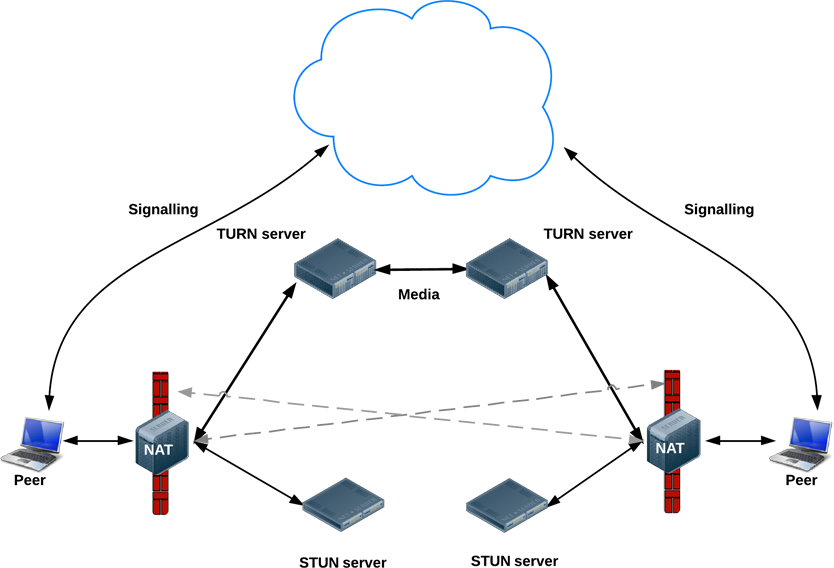
\includegraphics[width=12cm]{webrtc_turn}
\caption{Traversal Using Relays around NAT (TURN)}\label{fig:turn}
\end{figure}

WebRTC is the most appealing technical solution for the project proposed in this
thesis. The protocol will make sure that the players will be connected to the
game using the shortest possible network route therefore having the smallest
latency. In most cases players will be located behind the same NAT, and after
establishing a connection, no data will travel further than to the router.


% \subsection{Mobile devices Game Controllers} % game controllers + web

% \subsubsection{Native Apps}

% \subsubsection{Web Apps}

\subsection{Existing Solutions on the Market}

Even though WebRTC is a quite fresh technology, there are already plenty of
projects using it. Some of these projects are created by developers as part of
the Chrome Experiments\cite{chromeexperiments} project, in order to demonstrate
the technology and its capabilities. Two projects in particular are of interest
to this thesis as they represent the concept of a mobile phone being used as a
gaming controller. The following sections briefly describe the games and point
out things that may be applied to this thesis.

\subsubsection{Lightsaber Escape} % https://lightsaber.withgoogle.com/

The Lightsaber Escape\cite{lightsaber} is a small single-player arcade game
created by Lucasfilm Ltd in collaboration with Google in order to promote the
seventh film in the Star Wars trilogy. It requires a personal computer a
supported mobile device and an Internet connection. To play the game, the user
has to access the main page of the game
(\url{https://lightsaber.withgoogle.com/}) in a browser window on the computer
(figure \ref{fig:lightsaber_home}).

\begin{figure}[!h]
\centering
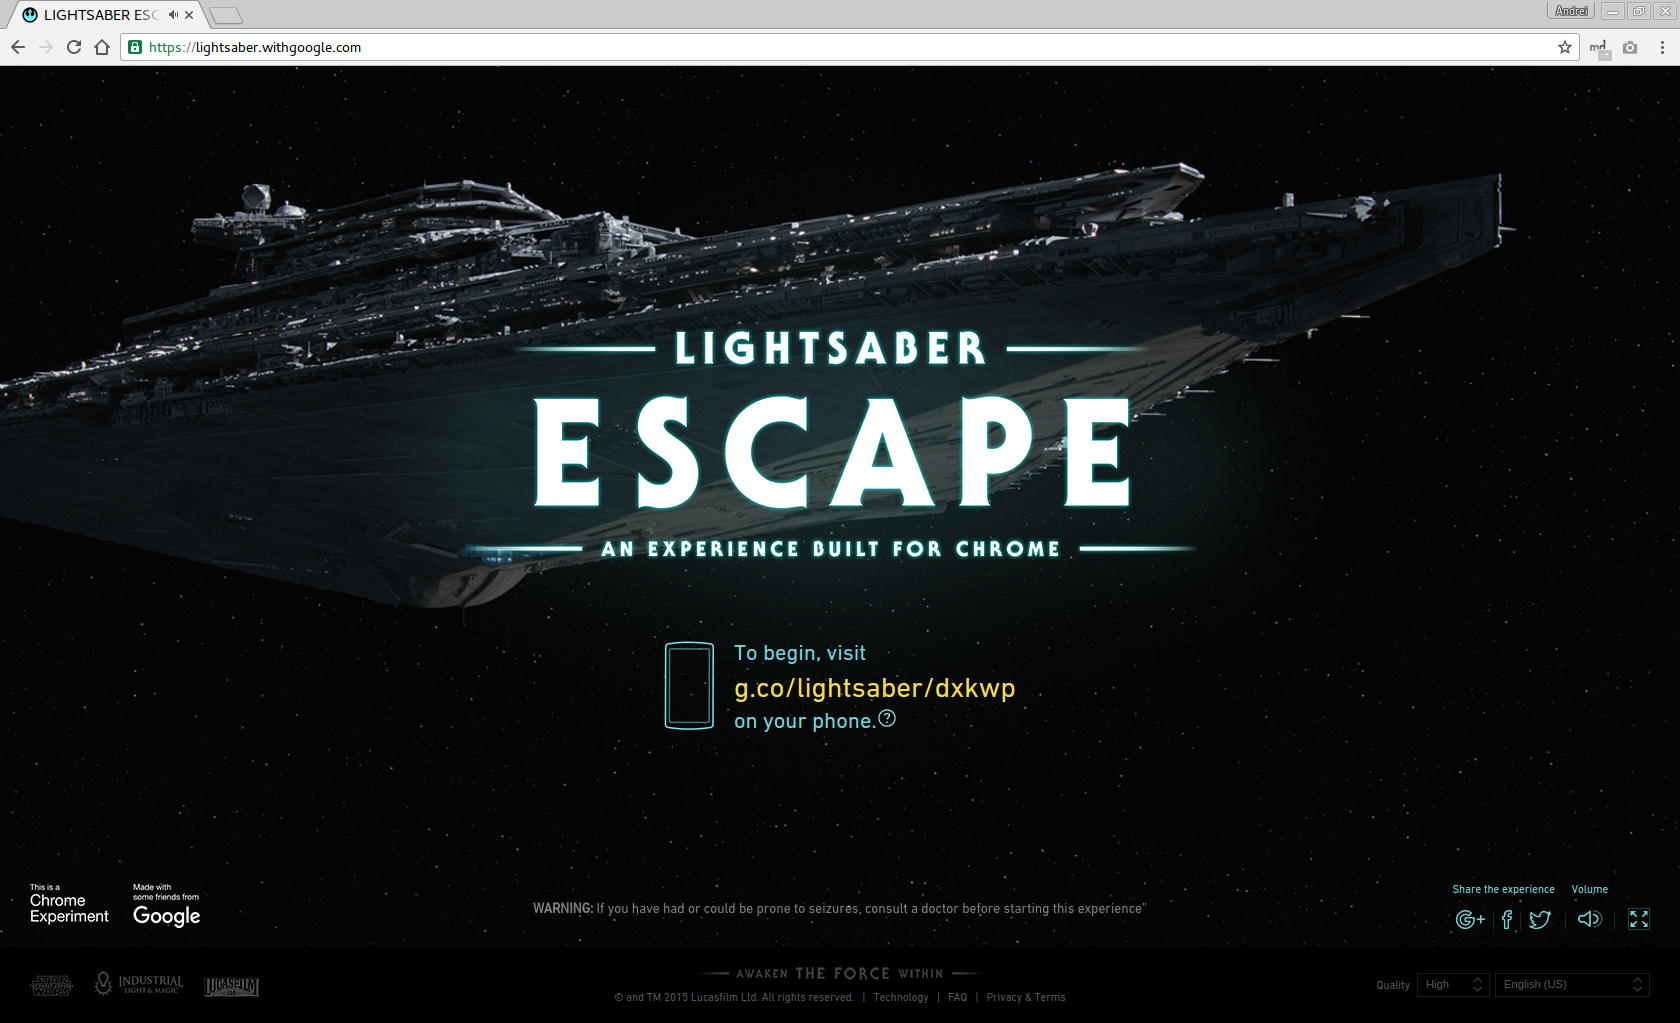
\includegraphics[width=10cm]{lightsaber_home}
\caption{Home Page of Lightsaber Escape}\label{fig:lightsaber_home}
\end{figure}

The user is presented with a short link that has to be entered in the navigation
bar of the browser on the mobile device. This brings the user to a page with
instructions to calibrate the device (figure \ref{fig:lightsaber_calibrate}).
During the calibration process, a connection is established between the phone
and the computer and the phone's gyroscope and accelerometer are calibrated.
After this procedure the lightsaber becomes active (figure
\ref{fig:lightsaber_active}):

\begin{figure}[!ht]
    \centering
    \subfloat[Calibration Screen\label{fig:lightsaber_calibrate}]{
      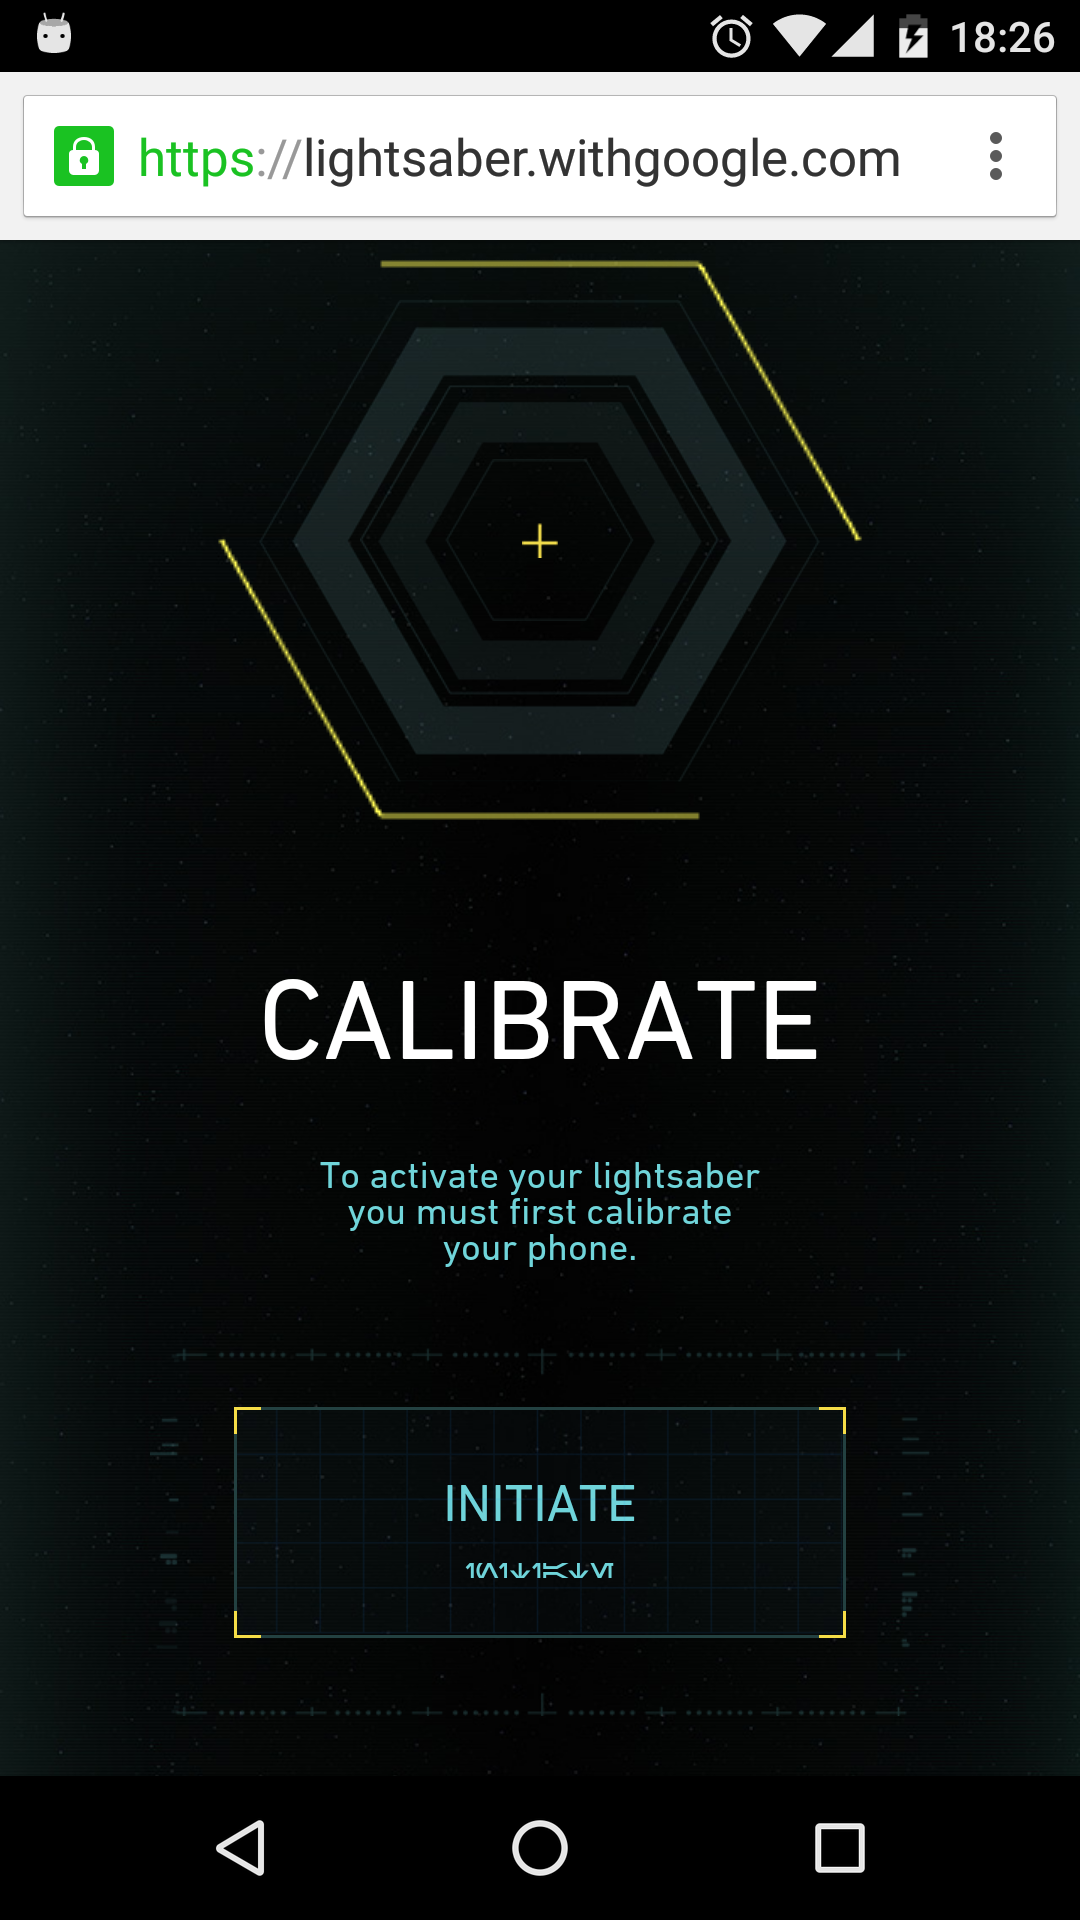
\includegraphics[width=0.25\textwidth]{lightsaber_calibrate}
    }
    \hspace{0.1\textwidth}
    \subfloat[Active Lightsaber\label{fig:lightsaber_active}]{
      
\includegraphics[width=0.25\textwidth]{lightsaber_active}
    }
    \caption{Lightsaber Escape as Seen on a Mobile Phone}
\end{figure}

With an active lightsaber, the player can start the gameplay, which consists of
dodging enemy laser blasts by controlling the lightsaber through movements of
the mobile phone. The player passes a couple of corridors in such a manner,
until he/she reaches a hand-to-hand combat encounter that resolves to the game's
finale.

\begin{figure}[!h]
\centering
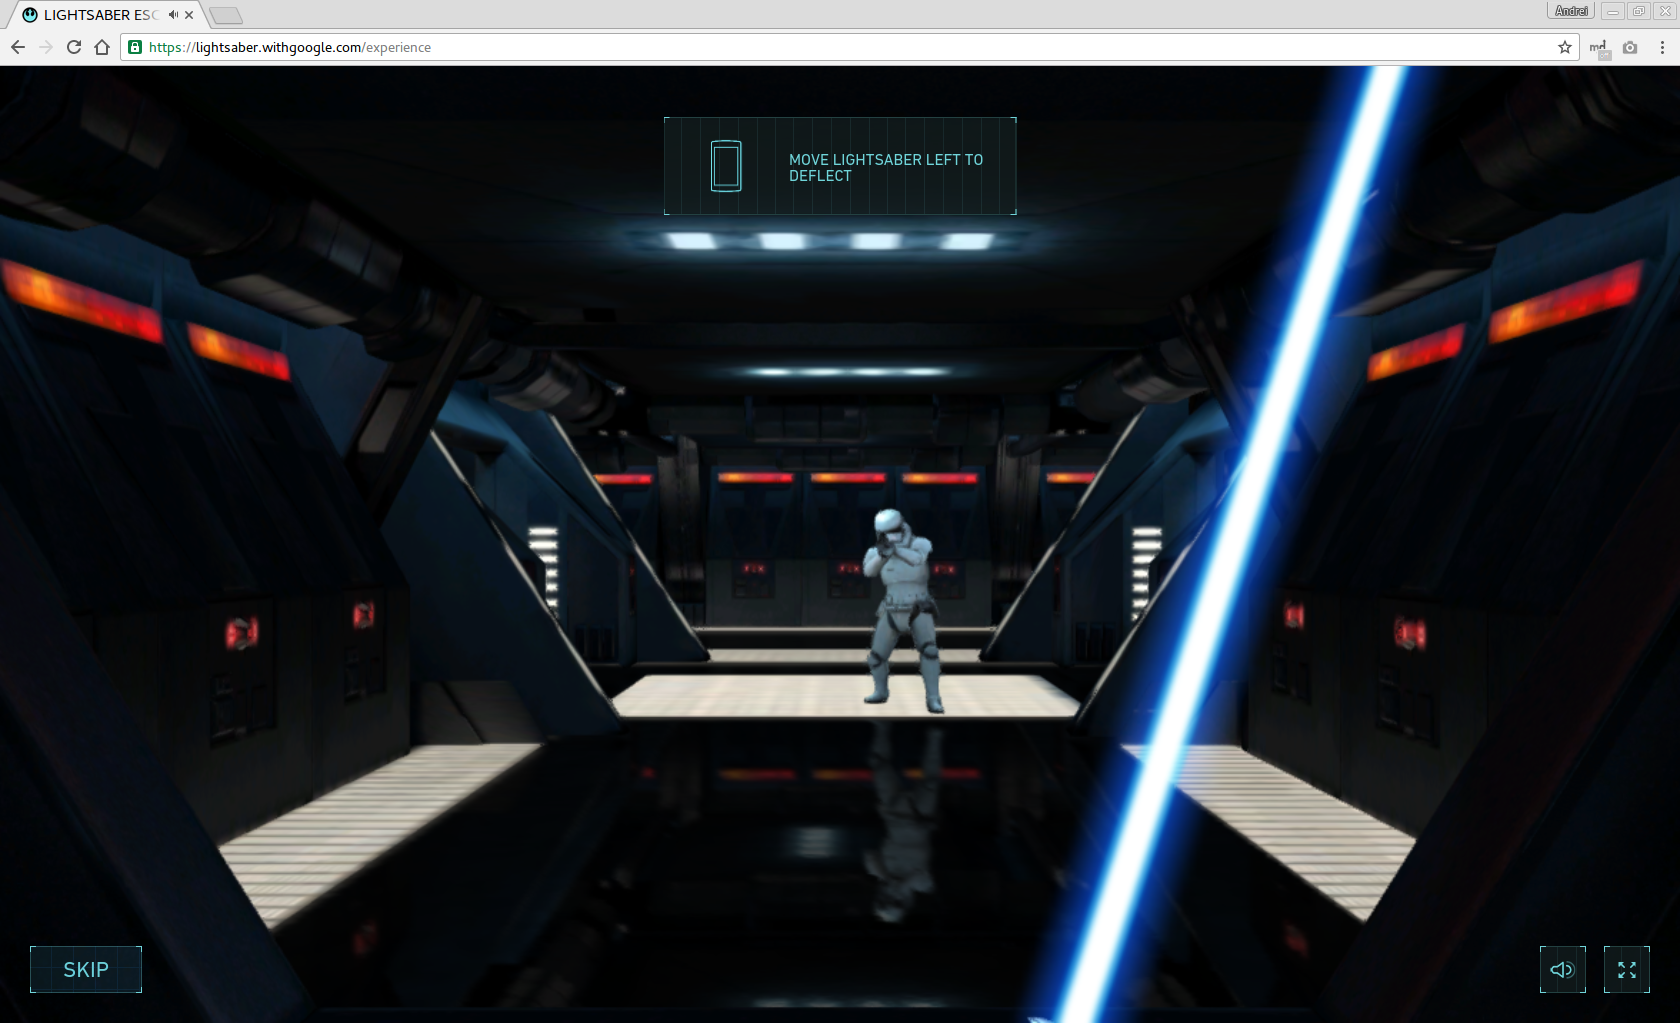
\includegraphics[width=10cm]{lightsaber_game}
\caption{Lightsaber Escape Gameplay}\label{fig:lightsaber_game}
\end{figure}

There are a couple of important things to note about this game. The clever way
in which are leveraged the motion-detection capabilities of a phone makes for a
really engaging experience, even though the whole gameplay lasts only about 5
minutes. If played on a powerful computer with a decent GPU, it could be noticed
that control mechanism is very smooth and responsive, this is thanks to an
efficient use of network traffic in the communication between devices. Overall
this game is a good way to promote a product using innovative technology and it
gives some hints on how to develop the project of this thesis.

\subsubsection{Super Sync Sports} % https://www.chrome.com/supersyncsports/

Super Sync Sports\cite{sports} is another Chrome Experiment with the same
concept of connecting a mobile phone to a computer in order to achieve an
interactive experience. This game has support for multiplayer gameplay for each
of the three game modes. Cycling mode is shown in figure \ref{fig:sports_game}.

\begin{figure}[!h]
\centering
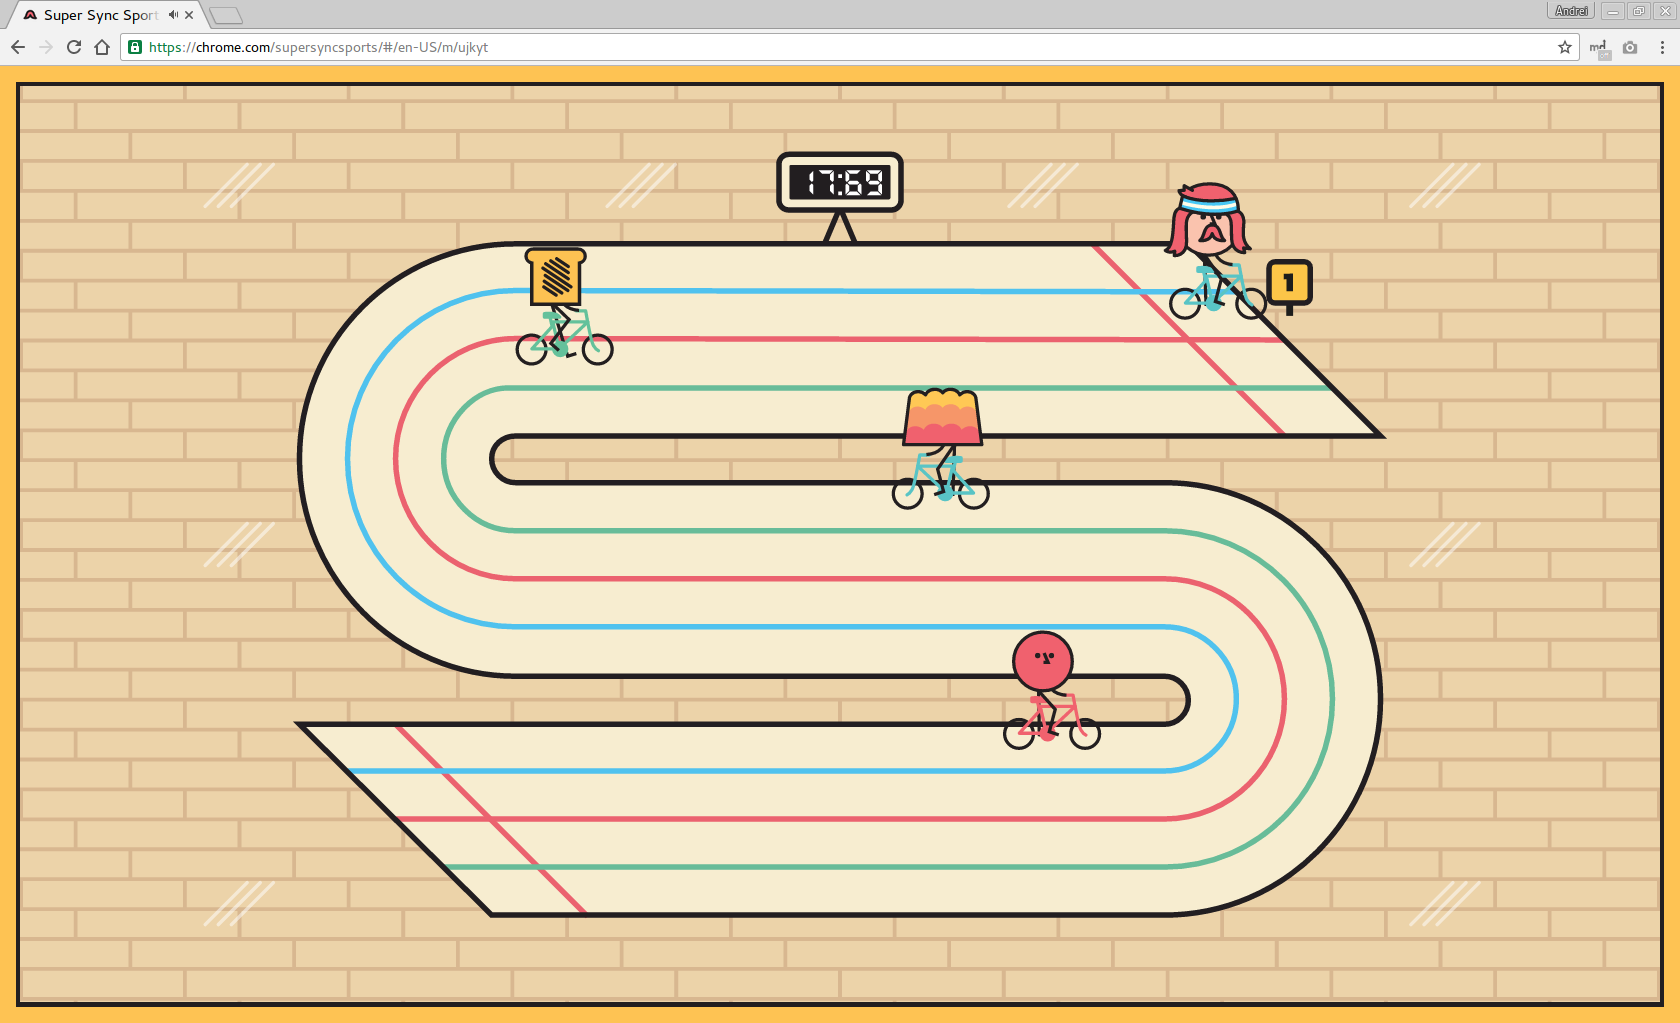
\includegraphics[width=10cm]{sports_game}
\caption{Super Sync Sports Cycling Challenge}\label{fig:sports_game}
\end{figure}

\newpage

Once connected, players can choose a character (figure \ref{fig:sports_player})
and use the controls on the phone (figure \ref{fig:sports_controls}) to race
with each other on a track. In contrast to Lightsaber Escape, does not use
motion-detection sensors of the phone, instead, the player activity is
controlled by sophisticated touch screen gestures.

\begin{figure}[!ht]
    \centering
    \subfloat[Character Selection Screen\label{fig:sports_player}]{
      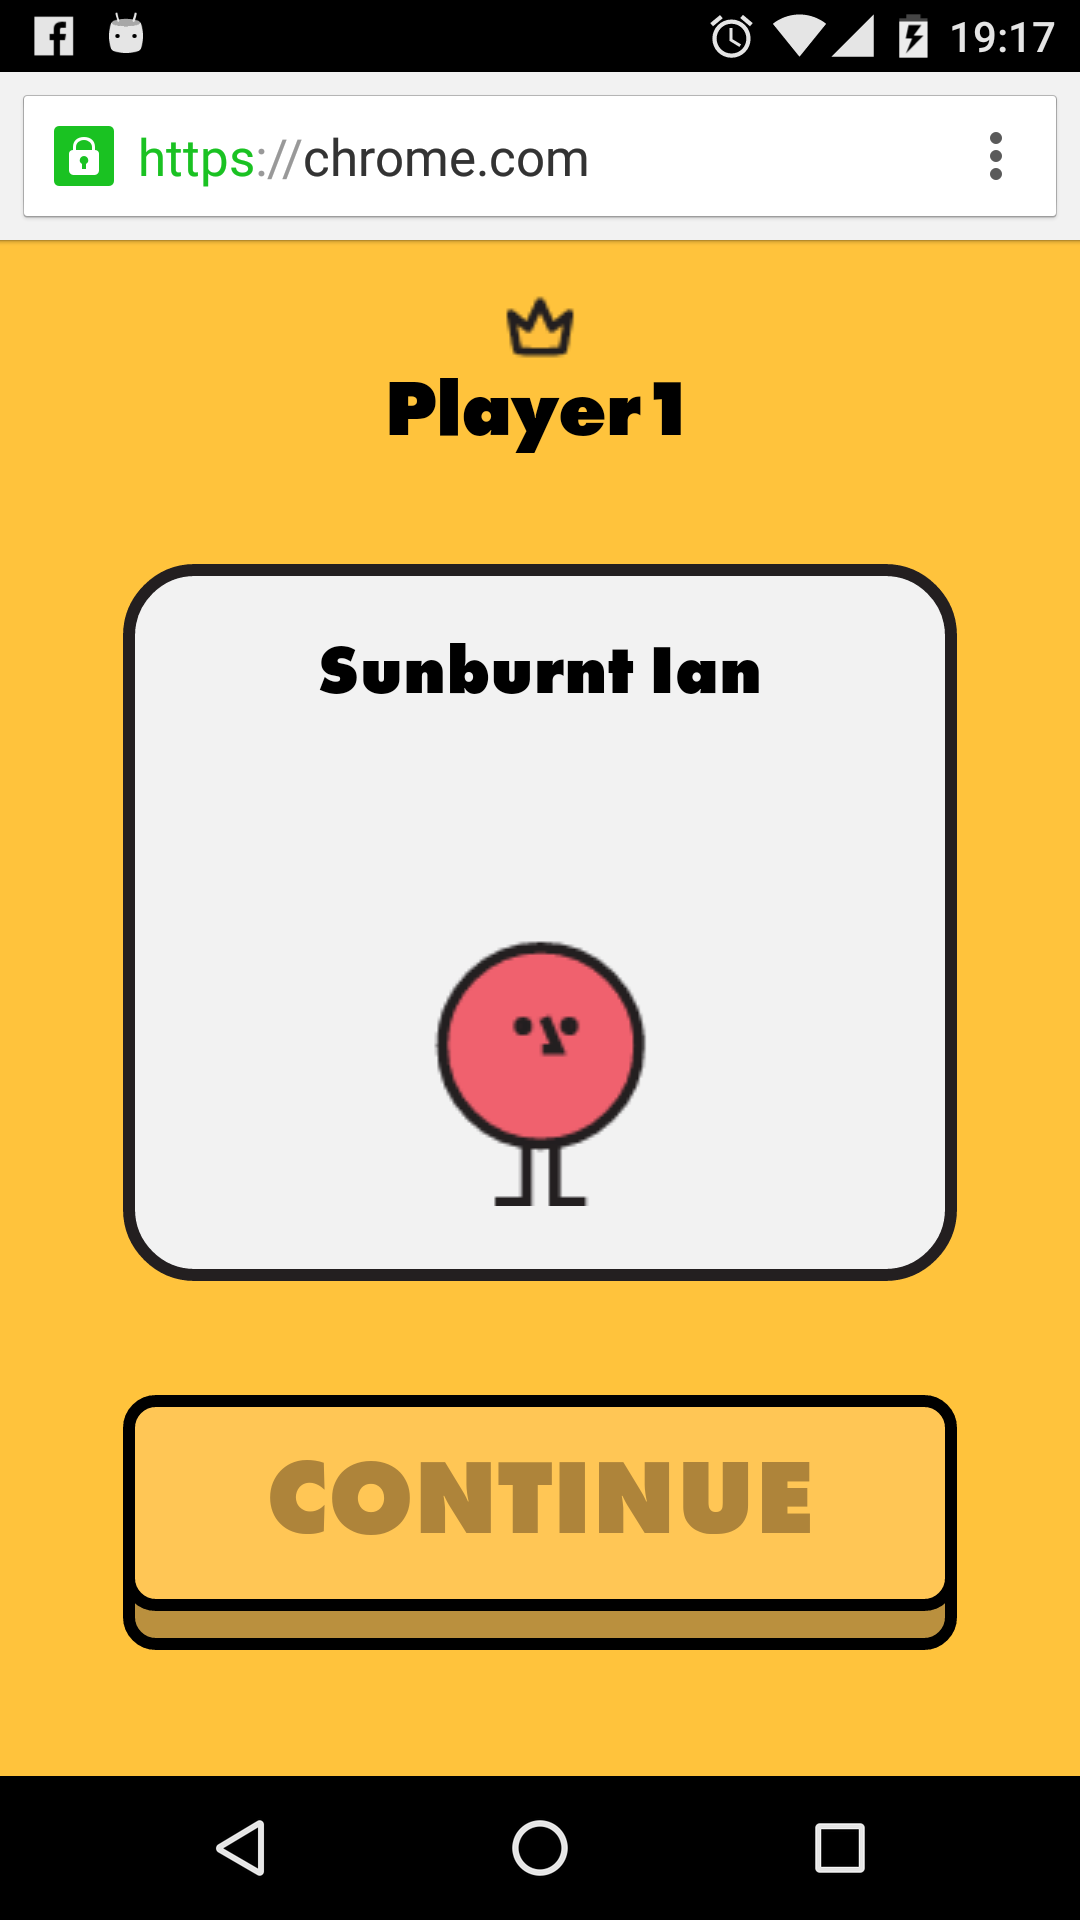
\includegraphics[width=0.25\textwidth]{sports_player}
    }
    \hspace{0.1\textwidth}
    \subfloat[Player Controls for Cycling Challenge\label{fig:sports_controls}]{
      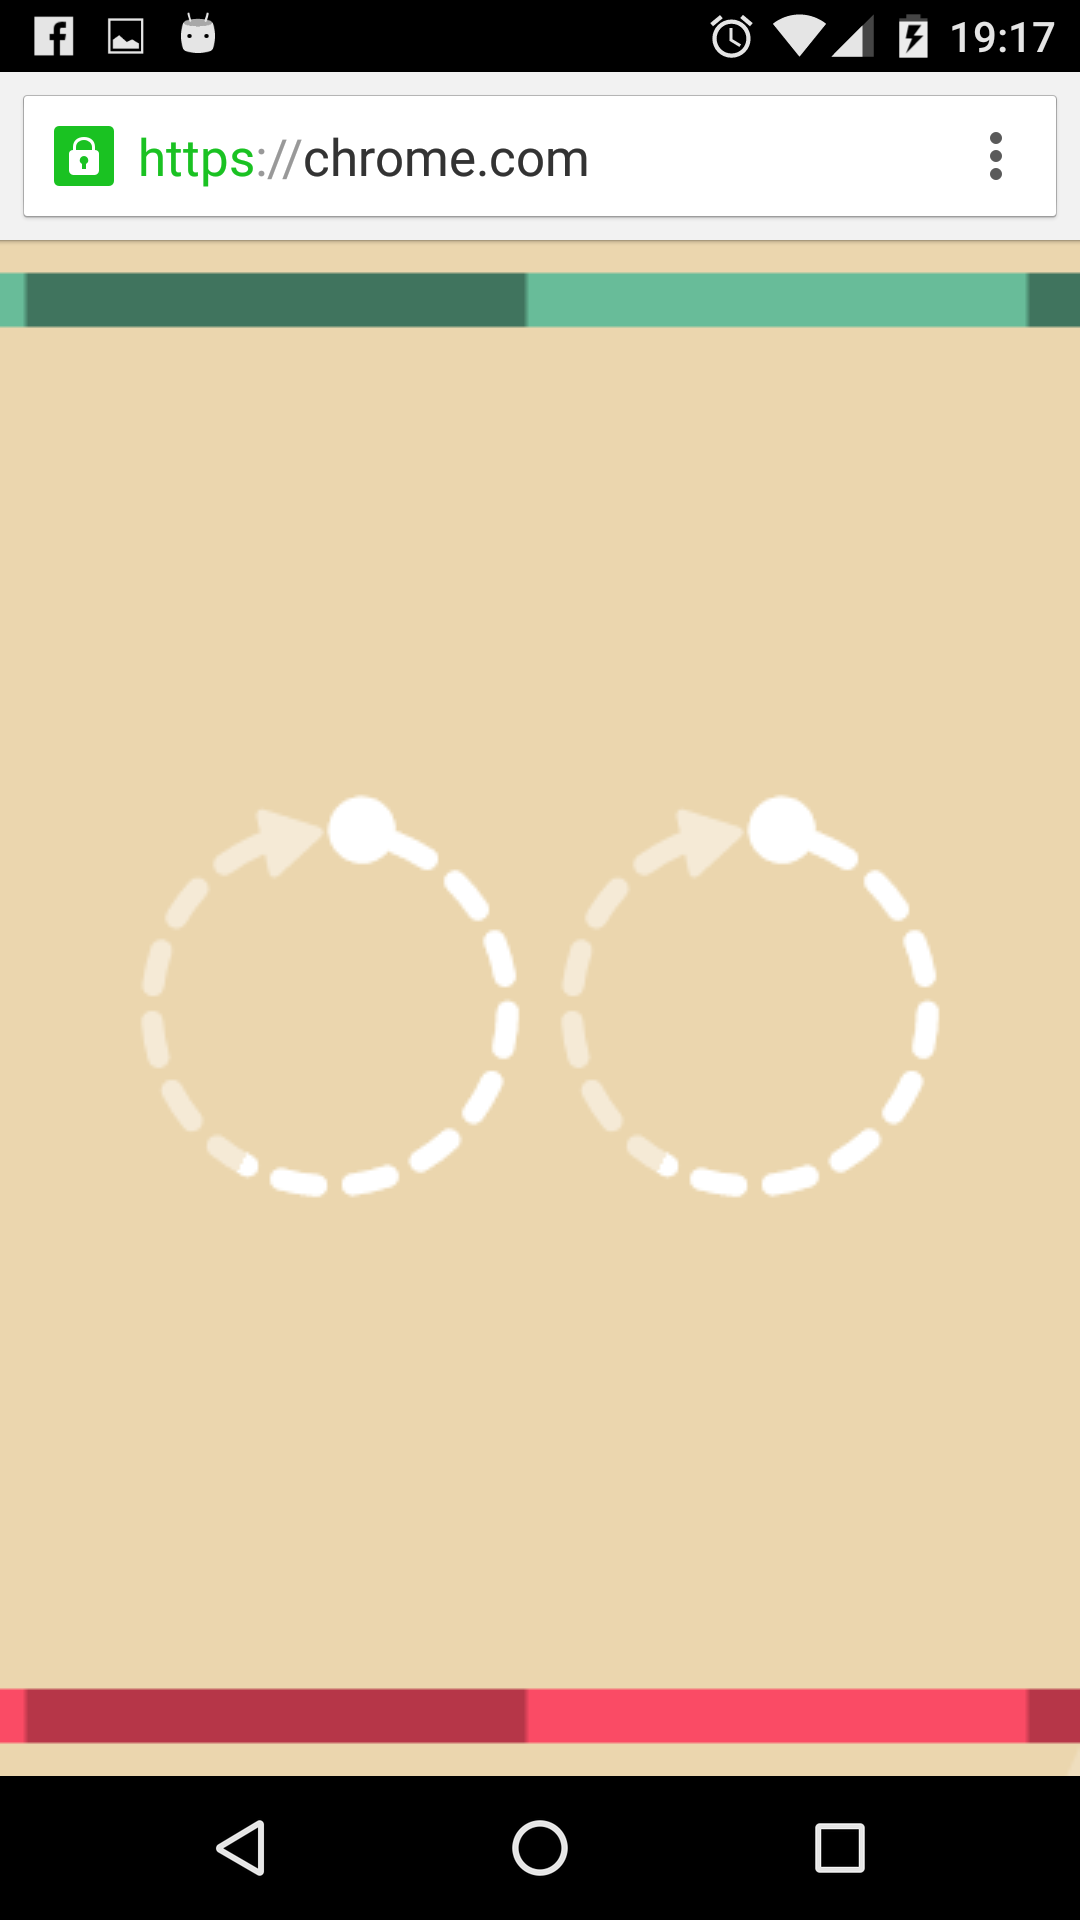
\includegraphics[width=0.25\textwidth]{sports_controls}
    }
    \caption{Super Sync Sports on a Mobile Phone}
\end{figure}

From the technical point of view, Super Sync Sports and Lightsaber Escape share
a lot of similarities like the connection procedures and the efficient use of
WebSockets technology. It is also interesting how Super Sync Sports delegates
things like character choice to the users phone rather than shows it on the
common game screen. This greatly increases the game configuration speed and
allows players to dive into the game right away.

\subsection{The 'Snowfight' -- Project Description}

Both of the games described above are great examples of interactive experience
achieved through the use of a mobile phone as a gaming controller. Under the
hood, they employ one of the two communication technologies be it WebSockets or
WebRTC.

The goal of this thesis is to replicate to some extent the functionality found
in these games using the available developer tools and to identify patterns and
techniques that can be used in similar projects. To achieve this, a multiplayer
game will be created on top of aforementioned technologies. The concept is
rather simple: players use their phones to connect to the game, they are placed
in an isometric environment stylized as a winter playground. The gameplay
represents a kind of 'death-match', in which players throw snowballs at each
other with the attempt to eliminate all enemies from the game before being
eliminated themselves.

The controller component of the game should consist of a gamepad-like system
rendered on the phone's browser with two main control elements: a trackball for
controlling player direction and velocity, as well as a button for throwing
snowballs. The communication between the controller and the game should be
efficient enough to allow up to 6 player to experience a smooth and responsive
gameplay, provided they are all connected to the same network.

Among other requirements, it should be possible to adjust the settings of
the player's avatar using the phone. Things that can be adjusted are the
player's on-screen name and the color of the avatar. Overall the game should
represent a functional prototype that would illustrate use the technology and
show potential of further development.


\subsection{Domain Analysis Conclusions}

As with any project, domain analysis is an important development step that is
able to prevent a great part of poorly made decisions. It can also boost the
creativity process as similar projects are analyzed and user opinion is
considered.

This chapter tried to identify a way to merge the domains of gaming and real-
time communication in an attempt to advance the concept of human interaction
with computers. A brief history of user interfaces and gaming devices evolved
into a discussion of how mobile phones could change the way people play games.

After that, two technologies where proposed to be used in order to achieved the
defined goal, mainly WebSockets and WebRTC, and a description of the thesis
project was provided in the context of two existing games that leverage the same
tools and technologies. As a result it is evident that for the purpose laid out
in the thesis, WebRTC is the best match, and should be used in the
implementation of the project.


\clearpage

\section{System Modeling}
\phantomsection

% TODO refactor diagram captions

\subsection{Use Case Layout}

\begin{figure}[!h]
\centering
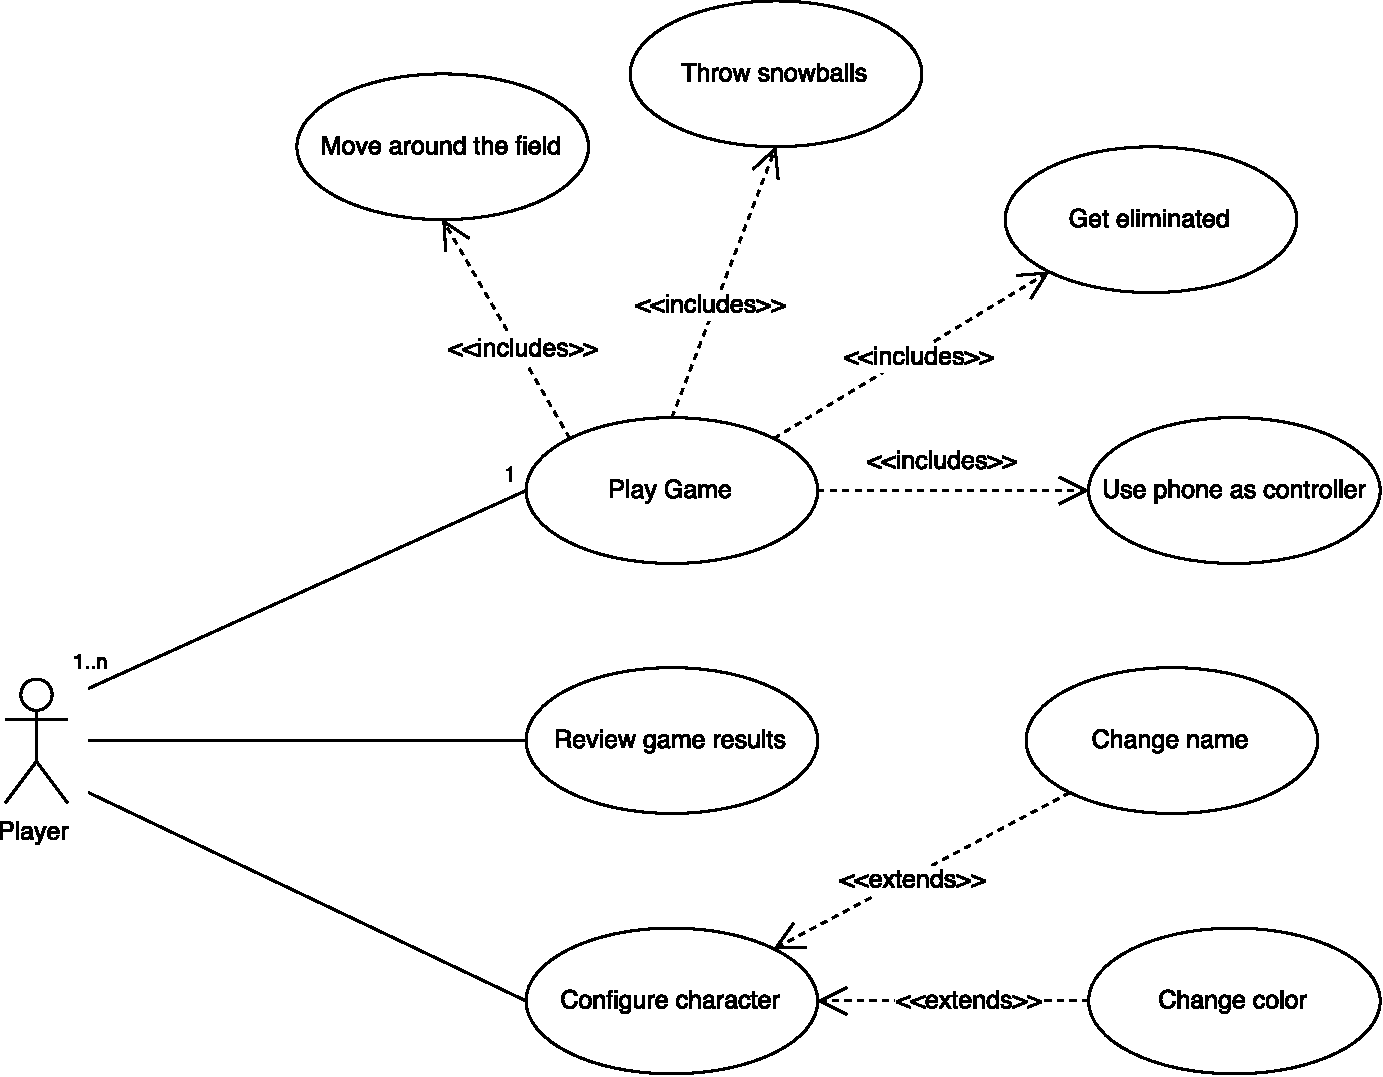
\includegraphics[width=15cm]{diagrams/usecase}
\caption{Use Case Diagram}\label{diag:usecase}
\end{figure}

\subsection{User Activity Graph}

\begin{figure}[!h]
\centering
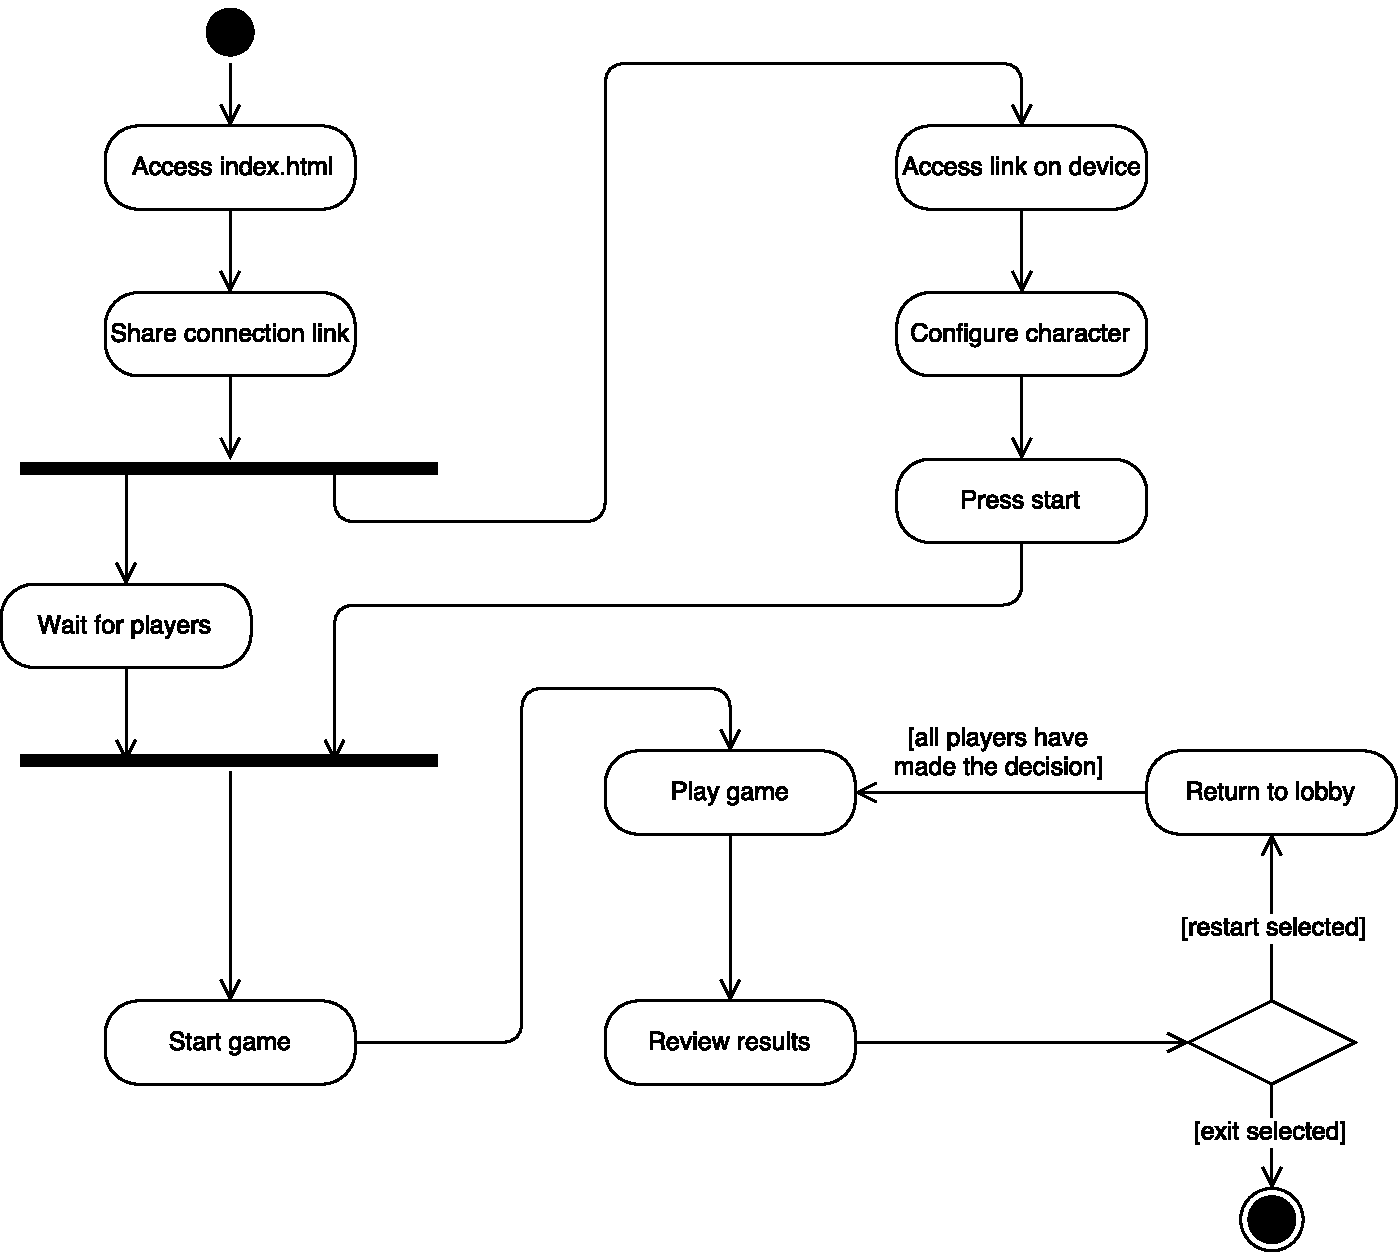
\includegraphics[width=15cm]{diagrams/activity}
\caption{Activity Diagram}\label{diag:activity}
\end{figure}

\subsection{Player States}

\begin{figure}[!h]
\centering
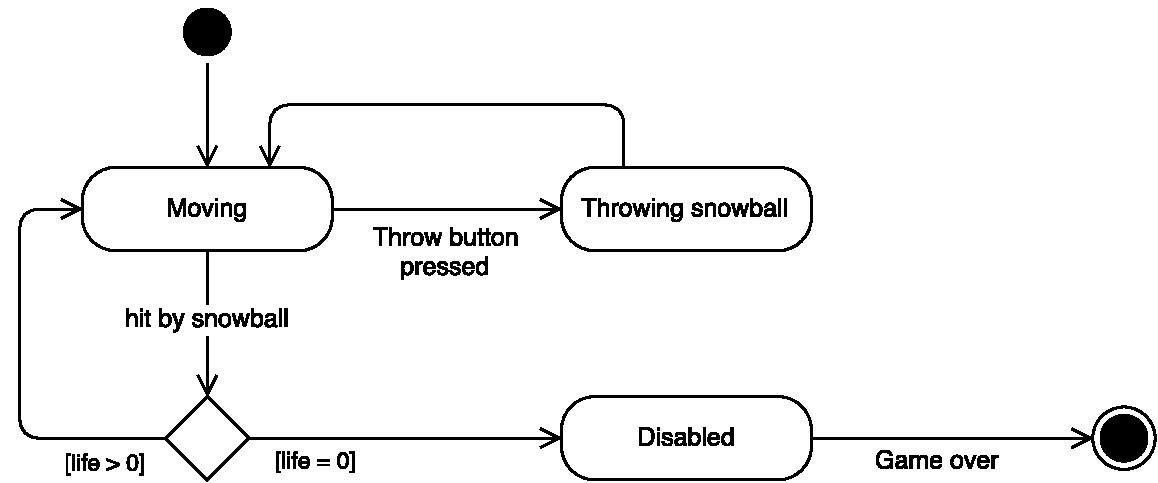
\includegraphics[width=15cm]{diagrams/state_1}
\caption{State Diagram}\label{diag:state_1}
\end{figure}

\subsection{High-level Game States}

\begin{figure}[!h]
\centering
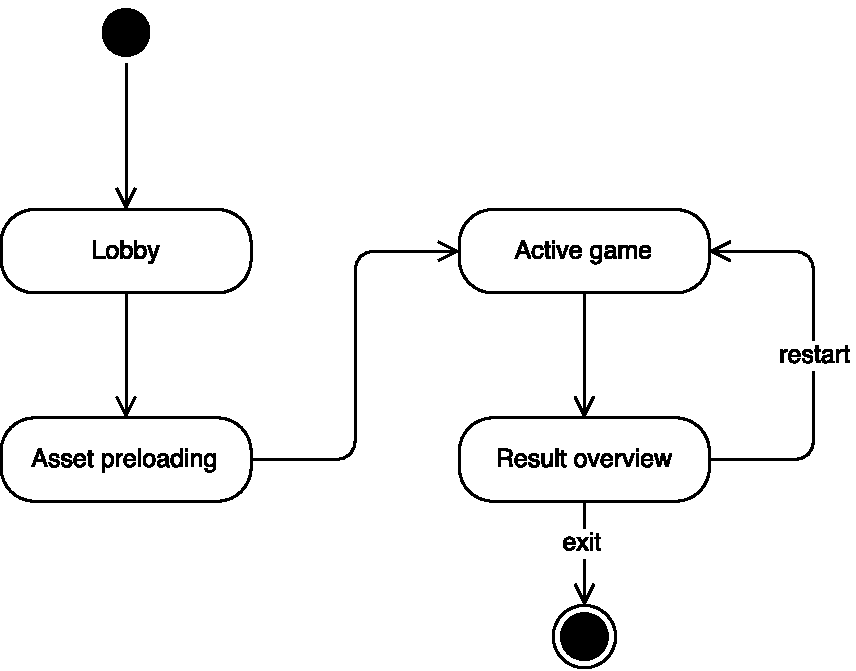
\includegraphics[width=15cm]{diagrams/state_2}
\caption{State Diagram}\label{diag:state_2}
\end{figure}

\subsection{Class Hierarchy of Game Objects}

\begin{figure}[!h]
\centering
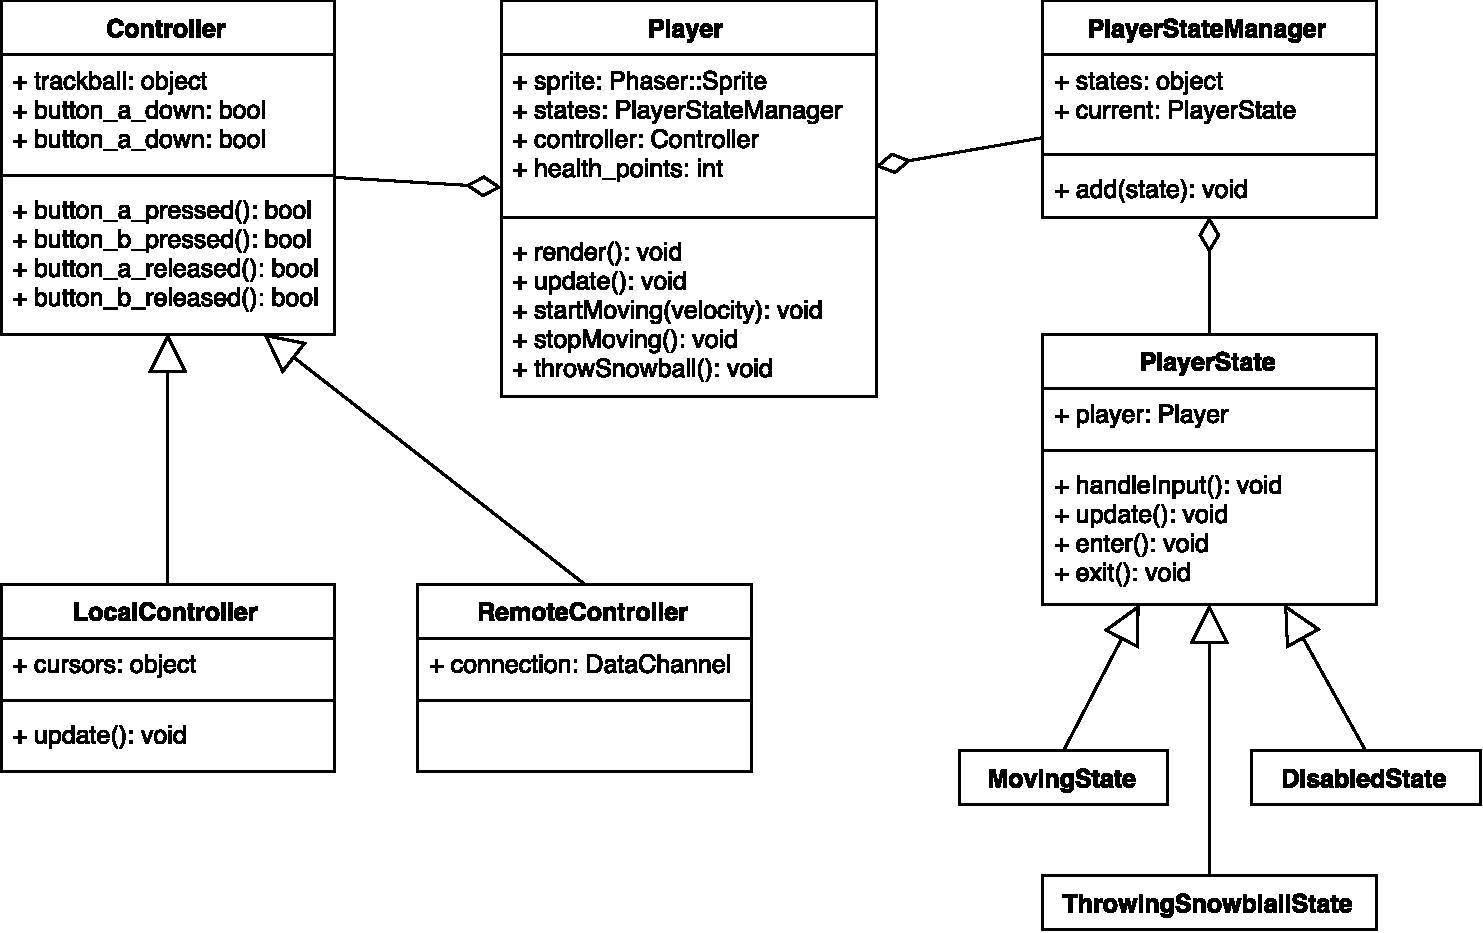
\includegraphics[width=15cm]{diagrams/class}
\caption{Class Diagram}\label{diag:class}
\end{figure}

\subsection{Components and Libraries}

\begin{figure}[!h]
\centering
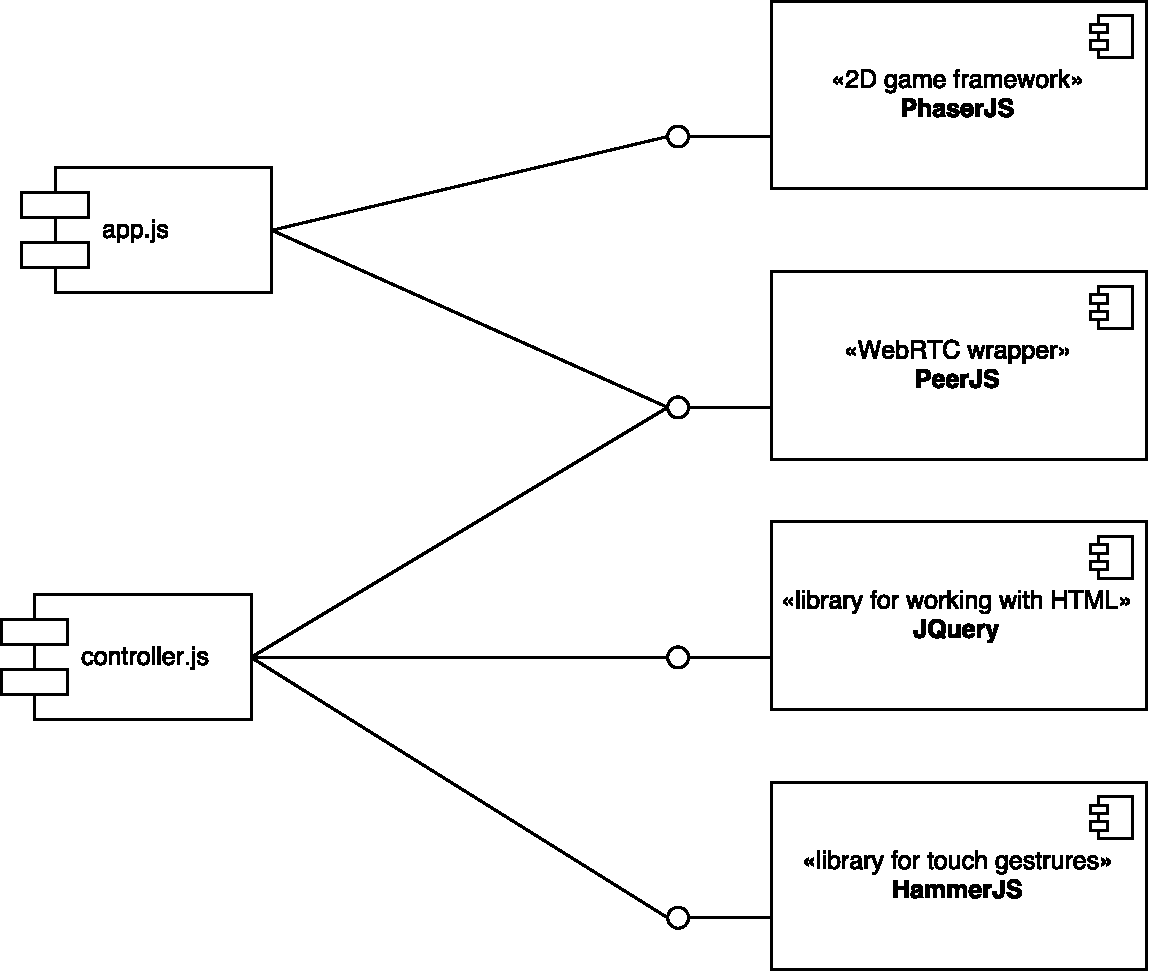
\includegraphics[width=15cm]{diagrams/component}
\caption{Component Diagram}\label{diag:component}
\end{figure}

\subsection{Deployment Setup}

\begin{figure}[!h]
\centering
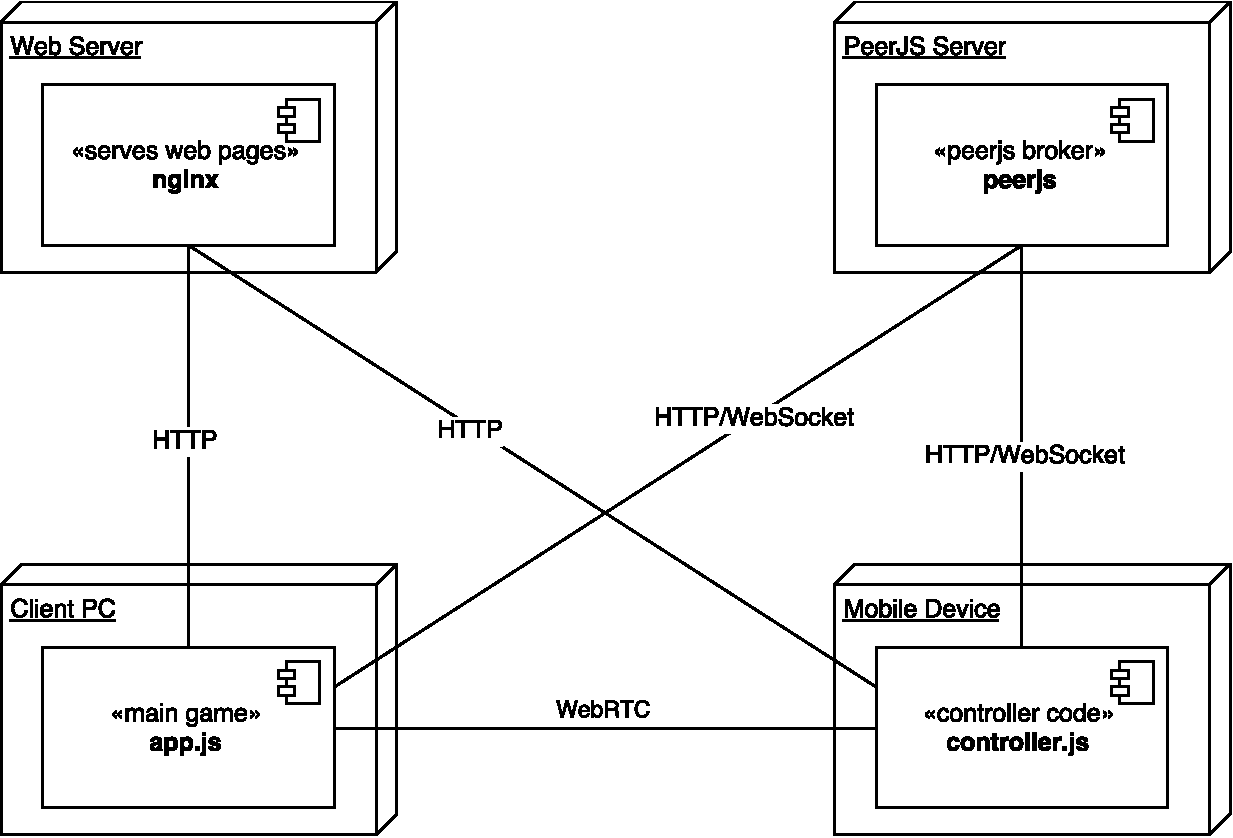
\includegraphics[width=15cm]{diagrams/deployment}
\caption{Deployment Diagram}\label{diag:deployment}
\end{figure}

\subsection{System Design Conclusions}

\clearpage


% IMPORTANT REMARK
% If your table of contents needs to be split in two parts (in order to
% accommodate the frame used for TOC) within the body text, right before the
% chapter/section that you want to be started on a new page, you should add:
\addtocontents{toc}{\protect\newpage}

\section{System Implementation Details}
\phantomsection

In this chapter is exposed a detailed description of the implementation details
of the thesis project. In the following sections are presented script excerpts
from both, the game and the controller parts of the system as well as the
communication code that links them together.

\subsection{Main Game}

The development of computer games is one of the most complex branches of the
software industry. Games encompass about a dozen different fields of mathematics
and computer sciences, to name a few, there is three-dimensional calculus,
differential calculus for physics, computer graphics, artificial intelligence,
game theory, etc.

Due to its complexity, game programming is among fields where the concept of
libraries and frameworks is more relevant than ever. Along the years, developers
around the globe have stumbled on the same problems in a recurring manner and as
a result, a lot of experience was gained which today is materialized as game
engines and development kits for all kind of platforms and types of games. In
this context it is much easier to prototype a game than it was ten years ago.

This thesis uses an HTML5 game framework called \emph{Phaser}\cite{phaser} which features a
rich set of tools that are required to build a 2D video game. This includes
rendering to an HTML Canvas or WebGL context, a physics engine, particle system,
asset management framework, sound engine, input handling, tiles, sprites and
much more. This framework was selected due to the ease and speed with which one
can develop a working prototype game that looks nice enough to be presentable.
On the other hand, 'Snowfight' is designed as an isometric game and doesn't meet
the main purpose of the framework, but this problem is easily solved by making
use of the framework's powerful plug-in system. The isometric plug-in extends
the Phaser capabilities like physics into the three-dimensional world and
perform an isometric projection on a two-dimensional canvas afterwards.

% TODO link to phaser isometric


\subsubsection{The Design of a PhaserJS Game}

In order to use a tool efficiently it is important to understand how it works.
The Phaser framework follows classic game programming patterns and has a
standard game loop which consists of three main steps:

\begin{description}

\item [Input handling] - the part where the user input is collected and
transformed into actions that are applied to the world whether it is changing
the direction and velocity of the player's movement or throwing a snowball

\item [Simulation update] - represents the process of updating the parts of the
system that do not directly depend on user input, like collision resolution,
object position adjustment depending on its velocity and such things as choosing
and applying the right frame of a sprite animation

\item [Rendering to screen] - consists of drawing all elements and textures on
an HTML5 Canvas or a WebGL context. When using Phaser, the programmer would
seldom override this step as the framework already does most of the work, with
of some rare cases when very specific adjustments and post-processing is needed

\end{description}

In Phaser games, the loop itself is hidden under the hood of the framework,
while a simple yet flexible interface is provided to the programmer to control
and fine-tune the steps specified above. In order to bootstrap a game it is
enough to instantiate a Phaser::Game object while providing the necessary
callbacks as in the example below:

\lstinputlisting[caption=Minimal Setup for a Phaser Game]{phaser_minimal.js}

The three methods in the example are not the only ones that can be overridden
and Phaser documentation list all of them and explains how they can be used to
customize the various use cases. The next section not only presents these
methods, it describes how different versions of them can be specified to be used
in different context, thanks to the concept of game states.


\subsubsection{Game State Management}

Every game is like a living system and everything a user sees happens inside a
game loop. Even if the screen shows the same static image, the game loop still
runs and refreshes the screen about 60 times per second. At the same time, most
games have a couple of situations when they behave completely different, the
most prominent example being the case of a three-dimensional shooter or racing
game when the user is in the menu compared to the time when he/she is engaged in
the game itself.

At the implementation level, it would be quite inconvenient to make the same
decision dozens of times per second, specifically the decision of choosing
whether to render the main menu or to compute the world physics and render the
game. The decision tree and, respectively, the chain of flow-control structures
grow as the number of these states that the game might be in, gets bigger and
bigger.

Software development techniques already include a solution to this kind of
situation in the body of a design pattern called the state pattern. \emph{The
Gang of Four}\cite{gof} describe a state object as one that encapsulates some
state-dependent behavior. This maps exactly to what happens in games, various
game states like main menu, active gameplay, cinematic cut-scenes, can be
modeled as objects that have specific implementations of methods for
rendering, performing updates and handling user input every frame.

The Phaser framework makes extensive use of the state pattern and gives
developers the opportunity to model their games as a series of interchanging
states with a set of predefined methods that are called by Phaser at specific
times in the main game loop and can be overridden in order to achieve certain
behavior. Some of the most commonly used methods of the abstract State object
are presented below with a small description of what are they usually used for:


\begin{description}

\item [init()] -- the very first function called when the State starts up;

\item [preload()] -- normally used to load game assets;

\item [create()] -- called when the State is ready to enter the game loop;

\item [update()] -- is for programmer's own use in order to define main game logic;

\item [preRender()] -- called after all Game Objects have been updated, but before any rendering;

\item [render()] -- called after the game is rendered, for final post-processing and style effects;

\item [shutdown()] -- will be called when the State is shutdown.

\end{description}


As the 'Snowfight' game is still quite small at this stage in development, it
features two main game states. Listing \ref{lst:preload_state} shows the code
that defines the 'preload' stage of the game. It is responsible for loading the
assets and bootstrapping all of the game systems like physics and plug-ins. For
this purpose it defines the \emph{preload} and \emph{create} methods.

\lstinputlisting[caption=Preload State, label=lst:preload_state]{preload_state.js}

The 'play' state, on the other hand, represents the description of the main
behavior of the game. It overrides the \emph{create}, \emph{render} and
\emph{update} methods and contains all the logic necessary to control gameplay
process.

\subsubsection{Player's State Machine}

Similarly to the architecture of the whole game, various subsystems can be also
modeled after the state pattern. Specifically the Player's behavior is heavily
dependent on the state that it is in at a given point in time. The need for a
stateful design aggravated at the point of developing the input handling system
as depending on the state of the player, user input had to be processed in very
different ways, for example when a player is disabled, movement controls have no
effect as opposed to the normal activity of the player.

The programming concept behind state handling of the player is similar to the
one used in the game object. A player object holds a reference to a state
manager that is responsible for keeping track of the current state as well as
adding and storing other states. A state object, at the same time, holds the
necessary logic to perform input handling or a player update. It also includes
the definition of the actions that have to be executed when a player enters or
exits a state. With this setup, when the game passes through the game loop and
a player receives a call of the update method, for example, it delegates it to
the state manage which in turn calls the method on the current state object.

Listing \ref{lst:player_states} presents the definition of a
dummy state as well as the code of the state manager.

\lstinputlisting[caption=Player States, label=lst:player_states]{player_states.js}

In his book on game programming patterns\cite{game_patterns}, Robert Nystrom
provides an excellent example of how games can leverage the science behind the
automata theory and how a nested chain of \emph{if} statements can be converted
to an elegant finite state-machine. The Player class in 'Snowfight' tries to
follow that example and model the object as a graph of states and transitions.

Diagram \ref{diag:state_1} from the chapter about system design shows the states
that a player can have (\emph{moving}, \emph{throwing} a snowball and
\emph{disabled}) and the various transitions that might happen between them. In
some cases a transition takes place as a result of an event or a condition that
evaluates to truth, at the same time some states transition to the next state
immediately after finishing their job. A good example of such behavior is the
transition from the player's state of \emph{throwing} a snowball back to
\emph{moving}, which happens right away without additional condition checks.

At the implementation level transitions are performed by the player state
manager and one can be triggered by a single line of code:

\lstinputlisting[caption=Moment of Transition to the Throwing State]{state_transition.js}


\subsubsection{Physics and Rendering}

An important part of a game is how it looks and feels. This mainly depends on
the physics and rendering systems of the game. Luckily, the Phaser framework
includes a decent physics engine that is capable of resolving rigid body
collisions and applying physical forces to objects. Rendering is also mostly
handled by the framework and the customization of the visual aspect of the game
consists of picking or drawing the right textures for the sprites.

The 'Snowfight' is an isometric game and in order to turn Phaser into a pseudo-
three-dimensional game engine, a respective plug-in is used. It extends the
coordinate space to a three-dimensional space and allows to perform collision
resolution in such conditions.

\lstinputlisting[caption=Isometric Plug-in Setup]{plugin.js}

Player animation is also an important aspect of the game. Phaser supports sprite
animation. In case case an animated object represents just a rectangle whose
texture is repeatedly changed in order to create the illusion of motion. It is
a widely used technique in 2D games. In case of games with an isometric
projection the sprites seem to gain an additional dimension.

\begin{figure}[!h]
\centering
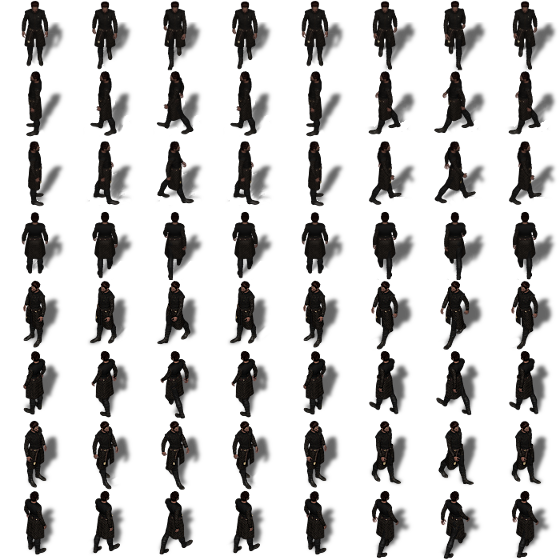
\includegraphics[width=10cm]{8frame_combined}
\caption{Player Spritesheet}\label{fig:knight_sprite}
\end{figure}

Figure \ref{fig:knight_sprite} represents a spritesheet with 8 looped animations
of character motion in 8 directions with 8 frames each. In order to load and use
these animations in the game it is necessary to tell Phaser the frame indices of
each animation and associate every batch with a name. The listing below
demonstrates this procedure:

\lstinputlisting[caption=Sprite Animation Loading]{character_sprite.js}

\subsubsection{Uniform Interface for Input Handling}

The development process becomes increasingly more difficult as the number of
moving parts in the system grows. It also becomes harder to debug and test
individual subsystems in isolated environments and in the case of 'Snowfight'
the development of the game was substantially slowed down by the fact that every
time the page was refreshed, it was necessary to reconnect the controller. In
addition, when some problems appeared it was not clear right away whether the
problem was in the game logic, in the controller code or in the communications
in-between.

One solution to the situation described above was to separate the game from the
controllers and develop it separately by providing the necessary input from the
local keyboard. This way, communication errors and bugs that concern controller
rendering would not stagnate the evolution of the core game.

From the implementation point of view the task required a unified interface for
all possible input sources, in this case only two of them. However, such an
approach opened opportunities to connect an artificial intelligence bot to the
abstract input device, which permits the addition to the game of non-player
characters (NPC) that would be controlled by the computer.

The base class of the Controller sets up the necessary variables and a set of
helper functions like the one in the listing below (\ref{lst:base_controller}),
that performs a check if a button was pressed just before the function call or
it was down all along.

\lstinputlisting[caption=Controller Base Class Highlights, label=lst:base_controller]{controller_base.js}

At the same time, listings \ref{lst:local_controller} and
\ref{lst:remote_controller} contain the specific bits of code that govern input
collection from the local keyboard and a remote mobile device respectively. The
main difference between the two is the fact that a local controller should be
update every iteration of the game loop in order to represent the accurate state
of the input device, while the remote controller is updated asynchronously by
means of callbacks.

\lstinputlisting[caption=Local Controller, label=lst:local_controller]{controller_local.js}

\lstinputlisting[caption=Remote Controller, label=lst:remote_controller]{controller_remote.js}


% \subsubsection{High-Level Game Logic}


\subsection{Controller}

The second major part of the system is the remote controller that is used to
operate a character on the main game screen. Following the motivations described
in the chapter on domain analysis, it represents a web page rather then a native
mobile application. As a result, it requires no prior installation procedures
because any modern mobile device is likely to have a decent web browser that
supports the necessary technological specifications.

The primary goal of the controller component is to provide an experience similar
to using a dedicated gaming device like a gamepad. The touch screen of a mobile
phone can be used to model various control elements like buttons and joysticks.
Even thought these fall short of three-dimensional tactile feedback, they can be
customized and optimized for an engaging and efficient gaming experience.
Moreover, modern browser APIs can trigger device vibrations of different
patterns in order to provide additional feedback.

The design of the controller and the kind of control elements it contains depend
on the type of actions they have to operate. In case of 'Snowfight', there are
two main activities that are controlled by the user, these are \emph{movement}
and \emph{throwing} snowballs. The mechanics of the game state that a snowball
is thrown in the direction of the player's current orientation. This means that
it is not necessary to have a control element like a joystick that would control
the direction, instead, a simple button should be enough to perform this action.
Movement, on the other hand, is a more complex activity and is controlled two
parameters, mainly, direction and speed. An ergonomic solution to this task is a
joystick-like control element. In the context of this system, the element is
called a track ball as it resembles a ball when viewed on the screen.

Figure \ref{fig:gamepad} represents a development version of the web-based
'gamepad' rendered on the screen of a mobile device in landscape mode. The left
side contains the track ball element for movement and the right side has the
button for throwing snowballs. The blue button at the top is a shortcut for
switching to full-screen mode.

\begin{figure}[!h]
\centering
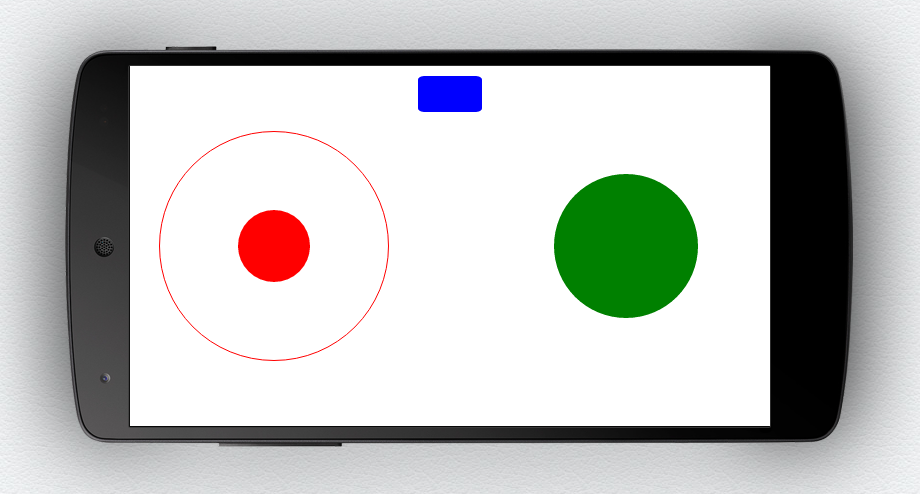
\includegraphics[width=15cm]{gamepad_nexus}
\caption{Web-based Gamepad}\label{fig:gamepad}
\end{figure}

As it is a web application, the controller and its elements are nothing but an
HTML5 document with appropriate styles and some scripts attached. The controller
layout is presented in the listing below. All elements are constructed of
\emph{div} tags that have specific class and id attributes in order to be later
processable by style-sheets and scripts.


\lstinputlisting[language=HTML, caption=HTML Layout of the Controller]{controller.html}

%\subsubsection{Mouse vs Touch Gestures}

\subsubsection{Track Ball Control Element}

In order to control character movement, it is necessary to represent some how
numerically this activity. In its simplest instance, movement on a plane has a
direction and speed, this maps perfectly onto the characteristics of a two-
dimensional vector, specifically its orientation and magnitude. Given a data
model, the next step is to come up with a control element that is able to
generate such data as a result of user input. On conventional gamepads this
feature is attributed to joysticks. They can be tilted to a certain degree
within a range in 2 directions, thus generating a set of 2D coordinates.
Joysticks also include a spring that returns them to the initial position in
case of no user input.

In the context of a touch screen device, it is not that simple to create a
moving stick, however, it is possible to draw a kind of ball that would track
the motion of a finger pressing on the screen and would reset to its initial
position when the touch motion is terminated. In addition, the web browser
interprets touch events in a different way from events generated by a mouse
device. Moreover, complex gestures like \emph{pan}, \emph{pinch zoom},
\emph{rotate} and \emph{swipe} require considerable effort in writing code that
detects these gestures, identifies the right type and fetches appropriate data
sets. Luckily, these problems have been solved by other people who developed
libraries specifically for such tasks. This thesis project makes use of the
HammerJS\cite{hammer} library that can recognize an handle gestures made by
touch, mouse and pointerEvents.

Gesture recognition is easily enabled by creating a \emph{Hammer} object
instance and specifying the HTML element that should trigger the events.

\lstinputlisting[caption=HammerJS Setup, label=lst:hammer]{hammer.js}

Listing \ref{lst:hammer} demonstrates how the ball element is passed to a
\emph{Hammer} object. After that, an option is specified to track \emph{panning}
motion in all direction. The \emph{pan} recognizer generates 3 kinds of events:
\emph{panstart}, \emph{panmove}, \emph{panend}. The listing above also shows how
callbacks are attached to each of the events in order to make use of the
information that is generated by them.


\subsubsection{Button}

The button part of the controller was considerably easier to implement as there
where no gestures involved. However, there was one aspect that had to be
clarified. When a button is pressed, its color should change to give some kind
of feedback to the user. This can be done through CSS pseudo-classes in a
trivial way, but it turns out such an approach has a drawback. There is a delay
of approximately 300ms between clicking on the button and the color change. In
case of usual websites it is almost unnoticeable, however, in case of games,
immediate feedback is crucial and the lack of it impacts severely the user
experience.

A logic workaround to this problem is to trigger the color change through
JavaScript code, by adding or removing the respective CSS class attribute, as it
is shown in listing \ref{lst:button}

\lstinputlisting[caption=Button Color Switch, label=lst:button]{button_color.js}


%\subsubsection{Responsive Design}

\subsection{Peer to Peer Communication}

Communication is the focal point of this thesis and makes all parts of the
system work as a whole. The game and the controller are nothing but simple web
applications and present no special value by themselves. In order to make them
communicate and interact, it is possible to apply several techniques. Most
things on the web communicate under a client-server architecture. This implies
there is an entity (a server) that orchestrates the whole process, it performs
all computations and provides services to the clients who always connect
directly to it. This project, however, has a slightly different twist to it.

The game and the controller are both applications are executed on the client
machine, moreover, there can be many simultaneous game sessions that must not
overlap in terms of communication. If the system were to employ the client-
server architecture, all the communications would have to be proxied through a
main server which would maintain control over all games and controllers.
Obviously, this model would be painfully slow and inefficient as large amounts
of data would have to travel long distances between devices and the server even
though the game computer and all the player are located in the same room and
connected to the same network.

In this context, the best option is a peer-to-peer communication model that
permits the exchange of information between parties directly, without the use of
intermediaries. Modern browser have recently introduced support for the WebRTC
technology that enables peer-to-peer communication with the use of a server only
for establishing the connection.


\subsubsection{Setting Up a Connection with PeerJS}

WebRTC programming interfaces are quite low level and performing the basic tasks
requires considerable effort from the developer. As with other software there
are libraries that have gathered the boilerplate code that is often used in
projects and hide it under simpler and higher level APIs. 'Snowfight' uses
PeerJS\cite{peerjs} which wraps the browser's WebRTC implementation to provide a complete,
configurable, and easy-to-use peer-to-peer connection API. Equipped with nothing
but an ID, a peer can create a P2P data or media stream connection to a remote
peer.

\lstinputlisting[caption=PeerJS Initialization, label=lst:peer_init]{peer_creation.js}

Listing \ref{lst:peer_init} shows how easy it is to initialize a Peer object. It
is enough to provide the address and port of a PeerJS server that will broker
the connections. A data connection is established simply by invoking the
\emph{connect} method on the Peer object. At the same time it is possible to
send arbitrary metadata that will be associated with the connection, in this
case it is the player's name which can be entered by the user. Once a connection
is open, it is trivial to send data over it:

\lstinputlisting[caption=Sending Data Using a 'DataConnection' Object]{peer_send.js}

When a controller initiates a peer-to-peer connection, the game lobby has to
catch this event and execute the necessary procedures in order to be able to
receive data. As many other things in JavaScript this is done by the use of
callbacks that are attached to specific events. Listing \ref{lst:peer_hub_init}
shows that every incoming connection object, that is intercepted by the game
while in lobby, is collected in a JavaScript array.

\lstinputlisting[caption=Connection Gathering, label=lst:peer_hub_init]{peer_hub_create.js}

Later on, at the initialization step of the game, every connection is attached
to a \emph{RemoteController} object, which in turn, sets callbacks (listing
\ref{lst:controller_callbacks}) that process incoming data and update the
internal state of the controller.

\lstinputlisting[caption=Controller Callbacks, label=lst:controller_callbacks]{controller_callbacks.js}


\subsubsection{Communication Protocol}

Establishing a connection is definitely not enough for an efficient and fruitful
communication. The chosen format of data that is to be exchanged between the
parties can heavily influence the flexibility and the performance of the system.
Devising a protocol is not a simple task because there are a lot of questions
that a developer should be able to answer before proceeding to the
implementation step.

Some of the things that should be clarified are listed below:

\begin{itemize}
\item what kind of data to transmit
\item how to order the data inside of a message
\item how to encode the transmission
\item how reliable should be the connection
\end{itemize}

The fact that a communication library is being used, greatly simplifies some of
the aspects of the protocol. For instance, PeerJS by default encodes all
messages in binary be it a string or a JavaScript object. The gaming context
also emphasizes performance over reliability, that is, if a message about the
current position of the trackball is lost, nothing catastrophic will happen.

The question that remains, though, is what kind of data should be sent from the
controller to the game and how should a message be formatted. At this point in
development, the system needs only two types of messages, one about the
trackball position changes and one about the changes in the state of a button.
These to types can be easily differentiated by a \emph{type} field in the top
level object of the message. In addition, a small number of message types does
not enforce a deeply nested structure. Listings \ref{lst:trackball_msg} and
\ref{lst:button_msg} represent examples of messages for trackball position
change and a button event respectively:

\lstinputlisting[caption=Trackball Message, label=lst:trackball_msg]{trackball_msg.json}

\lstinputlisting[caption=Button Message, label=lst:button_msg]{button_msg.json}

This protocol is by far not the best and the most efficient, but it works fine
for the current state of the system. At the same time, in case of further
development, it is certain that the message format will change drastically.

\subsection{Implementation Conclusions}

This chapter of the thesis gave an overview of the tools and techniques used
build all the parts of the system. It presented the Phaser framework and a
typical structure of a game that uses this framework. The sections about the
controller explained the motivation behind its components and control elements.
The final sections on peer-to-peer communication described the procedures that
where employed in order to establish a communication channel between the
controller and the main game. It also provided a brief description of the
protocol used to exchange information and control messages between the parties.

Overall, the technical side of the project is relatively straight forward and
does not contain scientific breakthroughs nor great innovations. On the other
hand, it represents an attempt to realize an already existing concept and
identify various pattern that can be reused in other projects on a greater and
more innovative scale.

\clearpage

\section{Economic Analysis}
\phantomsection

\subsection{Project Description}

The focus point of this thesis is the development of a toolkit that would
enable software engineers to create with ease web-based applications that
feature real-time communication with mobile devices and leverage all the
sensors and feedback elements that a modern smart-phone can deliver. In the
economic context, however, it is not enough to develop a framework, it is also
crucial to have a demonstration application that implements logic which uses
this framework, so that it can gain public attention and obtain necessary
financial investments to support its further development. The 'Snowfight' game
is a wonderful way to illustrate the power of real-time peer-to-peer
interaction between a desktop browser and a browser of a mobile device. It can
also effectively showcase the majority of the use-cases of the framework.

\subsection{Project Time Schedule}

In order to be successful, a project needs to have an effective development
methodology. Presently, \emph{Agile Software Development} gains popularity and
proves to be a flexible and robust way to create software. This methodology
implies an iterative and adaptive process of development and this in turn
influences the time table that has to be established.

\subsubsection{Objective Determination and SWOT Analysis}

The main objective of the project can be derived from its motivation. The
'Snowfight' should illustrate at its best the features of the toolkit
described in the thesis. The game should represent an isometric multiplayer
arcade in which participants can throw snowballs in each other and score
points. The players should control their characters via their smart-phones,
specifically through a web page rendered in the browser of the phone which
represents a some kind of game controller. The gameplay should feel very
responsive as if the player uses a wired gamepad.

Besides showing off technical features of the framework, the game should
appeal to potential players that would use it as an entertainment asset at
parties or team-building events. It should be engaging and well balanced as to
provide casual, yet challenging, and maybe even addictive, gameplay. It is
advisable for the controller part of the system be supported by most types of
mobile devices.

In order to get a better picture of the product and different paths of its
development it is a great idea to analyze the project from the perspective of
Strengths, Weaknesses, Opportunities and Threats, as it has proven to be an
effective technique in project management.

\paragraph{Strengths}

\begin{itemize}
    \item Intuitive user interface
    \item Multiplayer with up to 10 players
    \item Doesn't require any special programs to be installed
    \item Entertaining
\end{itemize}

\paragraph{Weaknesses}

\begin{itemize}
    \item The technology is available only on mid to high-end devices
    \item The game is somewhat bound by the limitations of the graphical framework
    \item Only one game mode
\end{itemize}

\paragraph{Opportunities}

\begin{itemize}
    \item Add several game modes
    \item Improve graphics art
    \item Use this project as a step-stone for another project
\end{itemize}

\paragraph{Threats}

\begin{itemize}
    \item Lack of visibility on the Internet
    \item Development of similar frameworks by other teams
\end{itemize}

\subsubsection{Time Schedule Establishment}

Most of IT projects' lifetimes consist of 5 basic steps: planning, research,
development, testing and deployment. These steps are in turn subdivided into
smaller parts in order to make the whole process manageable in terms of tasks.
Most of the time table will be allocated to the step of development and
testing as these are the steps with the most workload. Planning and research
by itself shouldn't take up too much time, as requirements usually evolve
during development, also research is a thing that usually never stops. The
development of the project can also be split in tasks that can be performed in
parallel thus minimizing the overall time. Total duration of the project is
computed using the equation \eqref{eq:duration}.

\begin{equation} \label{eq:duration}
D_T = D_F - D_S + T_R,
\end{equation}

\noindent where $D_T$ is the duration, $D_F$ -- the finish date, $D_S$ -- the
start date and $T_R$ -- reserve time. Table \ref{table:schedule} represents
the first iteration of the project schedule. The following notations are used
to improve readability: PM -- project manager, D -- developer, GD -- graphics
designer, SM -- sales manager.

\begin{table}[!h]
\begin{center}
\caption{Time schedule}
\renewcommand{\arraystretch}{1.5}
\begin{tabulary}{1\textwidth}{| C | C | C | C | C |}

\hline \textbf{Nr} & \textbf{Activity Name} & \textbf{Duration (days)} & \textbf{People involved} \\
\hline 1  & Project concept definition          & 5     & PM, GD, SM, D \\
\hline 2  & Market analysis                     & 10    & PM, SM        \\
\hline 3  & Domain analysis                     & 15    & PM, D         \\
\hline 4  & Product requirements specification  & 5     & PM, D         \\
\hline 5  & System modeling (UML)               & 10    & D             \\
\hline 6  & Graphic design                      & 10    & GD            \\
\hline 7  & Framework development               & 20    & D             \\
\hline 8  & Main game development               & 30    & GD, D         \\
\hline 9  & Validation of results               & 10    & PM, GD, D, SM \\
\hline 10 & Documentation                       & 5     & D             \\
\hline 11 & Deployment and testing              & 10    & PM, D         \\
\hline 12 & Active marketing                    & 15    & SM            \\
\hline 13 & Total time to finish the system     & 145   &               \\
\hline

\end{tabulary}
\label{table:schedule}
\vspace{-2.5em}
\end{center}
\end{table}

\subsection{Economic Motivation}

This section aims to give a perspective of the project from the economic point
of view. This includes the expenses and profits encountered as a result of the
project's activity as well as the various strategies of commercializing. All
the costs and prices are given in MDL (Moldavian lei) currency. Tangible and
intangible assets, indirect expenses will also be taken into account. One
important thing to mention is that the game is the fact that it is being
developed as an open-source project and it's primary goal is to popularize the
framework and toolkit underneath. Nevertheless, there are still opportunities
to commercialize the game, especially on the rising wave of the term
'Gamification' which gained substantial popularity lately in various
industries. Thus, the game in modified versions can be licensed to companies
that would like to 'gamify' their internal processes. Another monetization
model that might bring some profit and cover the development expenses is the
so called 'freemium' pricing model. This implies that the game should be
released for freeb with a limited set of features and the full package
of features would be unlocked to people that purchase a subscription of some
kind.

\subsubsection{Tangible and Intangible Asset Expenses}

The budget for the required tangible and intangible assets is shown in tables
\ref{table:tangible_assets} and \ref{table:intangible_assets}. Direct
expenses are presented in the table \ref{table:direct_expenses}.

\subsubsection{Individual Person Salary}

\subsubsection{Indirect Expenses}

\subsubsection{Wear and Deprecation}

\subsubsection{Product Cost}

\subsubsection{Economic Indicators and Results}

\subsection{Marketing Plan}

\subsection{First Clients}

\subsection{Economic Conclusions}






\clearpage


\phantomsection
\addcontentsline{toc}{section}{Conclusions}
\section*{Conclusions}



\clearpage





\addcontentsline{toc}{section}{References}
\printbibliography
\cleardoublepage


\end{document}
